%\documentclass[12pt,a4j]{jreport}
\documentclass[a4paper,12pt]{jreport}
%\usepackage[dvips]{graphicx,color}
%\usepackage{array}main
%\usepackage{amsmath,amsthm,amssymb}
%\usepackage{refcheck}
%%%%%%%%%%%%%%%%%%%%%%%%%%%%%%%%%%%%%%%%%%%%%%%%%%%%%%%%%%%%%%%%%%%%
%\usepackage{eepic,eepicsup}
\setlength{\columnsep}{4mm}
\setlength{\parskip}{1.4mm}

\usepackage[dvipdfmx]{graphicx}
\usepackage{url}

\usepackage[fleqn]{amsmath}

\usepackage{caption}
\usepackage{flushend}

%excel2latex用に追加
\usepackage{multirow}
\usepackage{bigstrut}


%筑波大学のフォーマットからコピー
\usepackage{times} % use Times Font instead of Computer Modern

\setcounter{tocdepth}{3}
\setcounter{page}{-1}

\setlength{\oddsidemargin}{0.1in}
\setlength{\evensidemargin}{0.1in}
\setlength{\topmargin}{0in}
\setlength{\textwidth}{6in}
%\setlength{\textheight}{10.1in}
\setlength{\parskip}{0em}
\setlength{\topsep}{0em}
%%%%%%%%%%%%%%%%%%%%%%%%%%%%%%%%%%%%
%% タイトル生成用パッケージ(重要)
%\usepackage{sie-jp-sjis}
\usepackage{sie-jp-utf}

%% タイトル
%% 【注意】タイトルの最後に\\ を入れるとエラーになります
\title{テスト対象とフォールトの知識を用いたブラックボックステスト手法の研究}
%% 著者
\author{湯本剛}
%% 学位 (2012/11 追加)
%\degree{}
%% 指導教員
%\advisor{}

%% 専攻名 と 年月
%% 年月は必要に応じて書き替えてください。
%\majorfield{△△△△}\programfield{□□□□}
\yearandmonth{20XX年 3月}
%%%%%%%%%%%%%%%%%%%%%%%%%%%%%%%%%%%%%%%%%%%%%%%%%%%%%%%%%%%%%%%%%%%%

\begin{document}

\maketitle
\thispagestyle{empty}
\newpage

\thispagestyle{empty}
\vspace*{20pt plus 1fil}
\parindent=1zw
\noindent
%%
%% 論文の概要(Abstract)
%%
\begin{center}
{\bf 概要}
\vspace{5mm}
\end{center}

%%%%%
\par
\vspace{0pt plus 1fil}
\newpage

\pagenumbering{roman} % I, II, III, IV
\tableofcontents
\listoffigures
\listoftables

\pagebreak \setcounter{page}{1}
\pagenumbering{arabic} % 1,2,3

%%%%%%%%%%%%%%%%%%%%%%%
\chapter{序論}
ソフトウェア開発の中の品質を確保する主要な技術として,ソフトウェアテストがある.
昨今のソフトウェアの複雑性と規模の急激な増加に伴い,求められるテストケースの数も増加の一途をたどっている.
ブラックボックステストの場合,ソフトウェアの規模とテストケース数の関係は,ファンクションポイント総計値の1.15乗から1.3乗となる.
開発プロジェクトのファンクションポイント総計値は1970年から2000年までの30年間で約10倍の増加を示している [2].
テストケース数の増加に対応するために必要となるテスト工数は,ソフトウェア開発工数の多くを占めるようになって来ている.
日本のソフトウェア開発において,ソフトウェアテストは開発工数全体の28%から35%を占めるという調査結果が出ている.
また,調査結果の中には,90%以上を占めるという事例もある[1].
ソフトウェアテストの活動のうち,テスト実行工程がソフトウェア開発のクリティカルパス上にある唯一の工程となる.
テスト実行の前にテストケースを開発し,実行するテストの全体像を示せると,効率のよいテスト実行を計画できる.
テストケースの開発はテスト工数全体の40パーセントを占めると言われている[TPINEXT].
これは,テストケースの開発に多くの人員が投入されていることを示している.
多数の人員がテスト開発の活動に投入されているにもかかわらず, テスト開発のための明確に定義されたルールがなく,個々の考え方に基づいてテストを開発することが多い.
これはテストケースの重複や漏れの原因となる可能性がある.
本研究では,テストケースを開発する際の重複や漏れを解決することを目的とし,テストケースを開発するための手法を検討する.2章では,研究対象であるシステムテストにおけるブラックボックステストにおける課題と先行研究を調査し,3章では,テスト分析手法の提案と実験による提案手法の評価を行なった.4章では,3章にて提案した分析手法の具体的な適用方法としてテストデータの入出力に着目した手法の提案と適用評価を行った.5章では,分析手法を適用する1つの領域で起きる、状態遷移の組合せによるテストケース数の爆発に対処し,重要なテストケースを抽出する方法を提案し,適用評価を行なった.
%%%%%%%%%%%%%%%%%%%%%%%
%%%%%%%%%%%%%%%%%%%%%%%
\chapter{ブラックボックステストにおけるテスト分析とその課題}
\section{本研究の対象となるテストケースの開発方法とテストのレベル}
\subsection{テストケースの開発方法}
テストケースを開発する方法は,ソフトウェアの構造を基にテスト設計するホワイトボックステストと,ソフトウェアの仕様を基にテスト設計するブラックボックステストに大別できる[2] .
ホワイトボックステストはテスト設計のベースがソースコードのようなテスト対象そのものとなるため,テスト対象プログラムの行を網羅,分岐を網羅といった具合にテストにて網羅すべきアイテムを明確に選択することが容易である.
網羅基準はテスト設計技法として提唱されている[2].
一方,ブラックボックステストでは,テスト対象そのものではなく,テスト対象の動作条件や振る舞いについて記述した仕様をベースにしてテストケースを開発する.
ブラックボックステストのテスト設計技法の中で、仕様に対する網羅基準は,ホワイトボックステスト同様数多く提唱されている[2].
しかし,ブラックボックステストは,テストベースがAUTの物理的な構造ではなく論理的なふるまいの記述であるがゆえに,テストを作るための詳細化が複数の解釈で行われることが多い[3][4].
%しかし,ブラックボックステストのためのテスト分析は詳細化に一貫性がないことが多く,それがゆえにテストケースの漏れや重複が起きることも多い.本提案では,テスト対象とフォールトを知識化したテストカテゴリを用いて一貫性のあるテスト分析手法を提案する.
結果的にテストケースの重複や抜け漏れを引き起こす可能性も高くなる.
本研究では,ブラックボックステストを対象とする.
\subsection{テストレベル}
ソフトウェアテストは,開発ライフサイクルの中で複数のテストレベルに分けて行われる.
複数のテストレベルは,図1で示すVモデルと呼ばれる技術面にフォーカスしたサイクルモデルにて表現することができる\cite{arnold1996software}.
各検証レベルはソフトウェア開発の段階的詳細化のレベルと対応している.
本研究は,複数のレベルの中で,赤枠で囲んだシステムレベルの検証で行われるブラックボックステストに焦点を当てている.
システムレベルのテストは,開発した単体のソフトウェアがすべて統合されるため,規模の増大と複雑性の増加の影響を直接的に受けるからである.

\section{テスト分析}
Vモデルであらわす各レベルにて行われるテストはそれぞれ,開発プロセスと類似したプロセスを持っている [4].
テストのプロセスは, 図2のようにテスト計画がVモデルの左側の活動と並行に行われ,その後時系列にテスト分析,テスト設計,テスト実装が行われた後,Vモデルの右側の活動の中で,テスト実行と終了基準の評価が行われる.
また,テストプロセスの中でもテスト分析,テスト設計,テスト実装の三つの活動はテスト開発プロセスとも呼ばれている[5] .
テスト設計の際には,テスト設計技法が適用できるサイズにテスト対象を詳細化することが必要となる.この活動はテスト分析と呼ばれている.
% ブラックボックステストを設計するベースとなる仕様とは,図1で示したVモデルの左側の成果物のことである.
% 各検証のレベルでテスト設計のベースする仕様はテストベースと呼ばれている[5].
% 本提案の対象となるV字モデルのレベルでは図2のsystem performance specificationがテストベースとなる.
% テストベースとなる仕様書は,その後の工程である設計やコーディングといった活動のために記載されるものであるため,テスト設計技法を適用する1つのアイテムに対する仕様が複数個所に分散して記載されてしまうことが多い.
% また,記述が自然言語であることも多く,条件の組み合わせや順序についての記述が不足していることも多い.
% テスト分析はこのようなテストベースに対して,何らかの考え方に基づき,テストにて網羅すべきアイテムを選択し,整理する活動である.
テスト分析は,図3で赤枠で示したとおり,テスト開発プロセス中の最初の活動である.
\subsection{テスト分析の課題}
テスト分析の活動の出力となるテスト条件は,機能,トランザクション,品質特性,構造的要素といった多くの側面の総称であるため,各側面の関係を整理するための構造化が必要である.
しかし,テスト分析におけるテスト条件群の構造化は,研究や実務においても,経験則や個人の考え方に基づく構造化に留まっている [6].
一般的には,テストベースを表1のように大項目,中項目,小項目と詳細化していくことが多い.
この方法は,詳細化する際の各分類項目に明確なルールが定義されていないため,個人毎の何かしらの考え方で詳細化するための分類を決めていくことになる.
そのため,分類にばらつきが発生し,同じテスト条件が複数の階層に現れてしまったり,同じ意味のテスト条件が別の名称で選択されるといった混乱が起きてしまう.

この結果は複数の個人がそれぞれ複数の結果に到達することを示している.
%The different results mean a great variance in test conditions determined through test analysis.
複数の結果とは,テスト分析を通して特定したテスト条件にばらつきがあることを意味している.
%Thus, when the test analysis is performed by many individuals there is a high chance for test conditions to either be duplicated or even missed out entirely.
したがって,テスト分析が多くの人たちで行われるときには,テスト条件の重複,もしくは完全に抜け落ちるといった可能性が非常に高くなる.
\subsection{ブラックボックステストにおけるテスト分析の先行研究}
ISTQBでは,テスト分析を実行するための要求事項や必要性は述べている.
けれども,テストベースを分析していくためのアプローチは定義されていない.
これは,Ostrand [8], Grindal [9]などのテスト開発に関する先行研究でも同様である.
更に言うと,G.J.MyersやB.Beizerといった先行研究の多くは,テスト分析にてテスト条件が特定された後に適用されるテストパラメータの設計に焦点を当てている.
そのため,テスト条件は,すでに全て準備されたと言う前提になっている.
%Some studies on the test analysis method have also been proposed by Nishi [12], Akiyama [13], etc.
テスト分析手法に関する研究は,Nishi [12], Akiyama[13]などがある.
%While these studies look at the logic of analyzing AUT, they have little focus on how effective these methods actually are in reducing duplication and missing test conditions when working with more than one person.
それらの研究はテスト分析手法の論理に着目をしているけれども,複数の人数でテスト分析を行う際のテスト条件の重複と欠落について,手法を適用すると実際はどの程度効果的であるかについては,大きく着目していない.


%%%%%%%%%%%%%%%%%%%%%%%InSTA2016の論文
\chapter{論理的機能構造を使ったテストケースの特定方法}

%\section{VARIABILITY OF TEST ANALYSIS RESULTS}

\section{テストカテゴリベースドテストのアプローチ}
本章で提案する分析手法は,図~\ref{fig:D-3-Fig3}の論理的機能構造基づいてフィーチャをMECE(互いに相容れなくて完全に徹底的)な方法で分解して,テスト条件を特定する [16].
図~\ref{fig:D-3-Fig3}に示す各箱が,各フィーチャに要求されるテスト条件を特定する有用なガイドとなる.
\begin{figure}[h]
  \begin{center}
  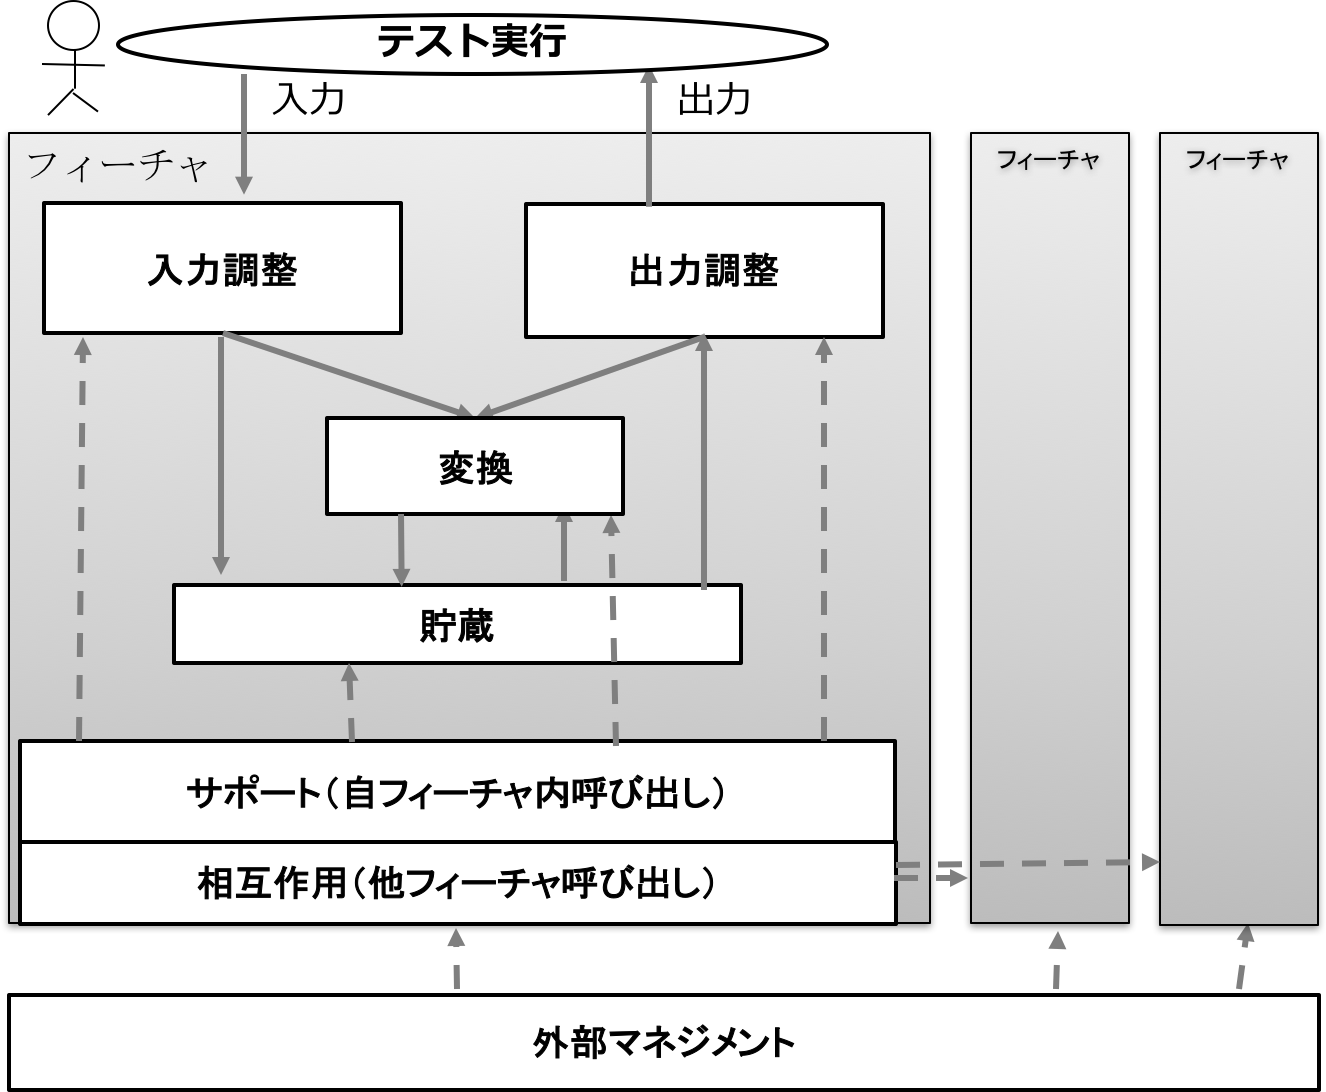
\includegraphics[width=12cm]{./image/D-3-Fig3.png}
  \caption{MECEにフィーチャからテスト条件を識別する方法}
  \label{fig:D-3-Fig3}
  \end{center}
   \end{figure}
%We can posit the hypothesis that by implementing a set of rules it will be easier to determine the necessary test conditions to ensure the appropriate testing takes place. The following issues currently make this difficult:
%テスト分析のルールを導入すると,テストに必要なテスト条件の特定が容易になるという仮説を立てている.現状,次に示す課題はテスト条件の特定を困難にしている.
%\begin{enumerate}
%\item 明白に必要だと思われる仕様の一部分が記述されていない.
%\item 機能間の組み合わせでどのように振舞うかといった仕様は,ドキュメント中の該当する単一のセクションには完全に記載し切れていない.
%\end{enumerate}

 論理構造は抽象的な概念であるため,各個人の解釈に違いが出る可能性がある.テスト条件の特定に一貫性を持たせるため, 論理構造に対してAUTに特化した名前付けを行う.
%In order to have a consistent interpretation of determining test conditions, a name specialized for the AUT is put in each box of the logical structure. This is called Test-Category.
名前付けしたものをテストカテゴリと呼ぶ.テストカテゴリはテスト条件を特定するための有用なガイドである.
%Test-Categories can be a useful guide for determining test conditions, including specification-items, expected results, and test parameters, from each feature.

更に,このテスト分析手法では,テストベースからテスト条件を特定するステップを下記に示す手順にて実行することを推奨している[6].
%Step1: Select feature to be tested
%Step2: Design Test-Categories
%Step3: Select and organize specification-items and expected results using Test-Categories
%Step4: Select and organize test parameters

\begin{description}
\item[Step1] テスト対象のフィーチャを選択
\item[Step2] テストカテゴリの設計
\item[Step3] テストカテゴリを使い仕様項目と期待結果を選択,整理する.
\item[Step4] テストパラメータを選択し,整理する.
\end{description}

多くのテスト開発に従事するテスト担当者が上記のステップに従うと,その全てのテスト担当者は,同じルールに沿って各自の仕事を実行できる. 結果として,開発されたテスト条件のまとまりは,より包括的で,重複が含まれない.これは総合的に見て高いテストカバレッジを確かにし,高品質のテストを提供することにつながる.これは本手法の主たる効果となる.

%Furthermore, there are three benefits to this procedure:
更に,この手順には3つの効果がある.
\begin{enumerate}
\item この手順は,本手法で提案しているテスト条件の構造をベースにしている [6]. テストベース内の要素は,仕様項目,期待結果,テストパラメータに分類できる.この手順を通して,各要素は1つずつ順番に特定,選択する. テスト分析にて同じロジックと手順で作成し,同じカテゴリに分類できた各メンバーの最終結果の可読性が向上する.
\item テストカテゴリに対する合意形成によって,チームメンバは仕様項目の特定と選択が容易になる.
\item 本手法は体系化され,標準化され,進めていくのか用意になるため, テスト担当者がテスト分析を繰り返すことができるようになる.
\end{enumerate}

%Verification experiments were performed to prove the effectiveness of this prevention.
テストカテゴリの効果を証明するために,検証実験を行った.

%\section{Remarks from the Verification Experiments検証実験からの考察}
\section{検証実験からの考察}
\subsection{検証実験の手順}

%The verification experiments were conducted during workshops. In these workshops it was explained that a test development process is required in order to derive test cases.
検証実験は,ワークショップを通じて実施した.ワークショップでは,最初に,テストケースを導出するためにはテスト開発プロセスが必要であることを説明する.
%After showing the test basis for a particular exercise, the test analysis was carried out. The participants were grouped into teams of four or five members.
そして,演習に使うテストベースを示し,テスト分析を実行してもらう.
全出席者がテスト分析の最初の結果を理解した後, テスト分析手法を説明し、手順に沿って再度テスト分析を実施する.
検証実験は3回実施した.
1回目,2回目の実験では,1回のワークショップには上記の4時間で上記の全手順を実施した.3回目の実験では、再度音楽再生機器をAUTとして利用した.しかし,チームにわかれて実験結果を得るのではなく,実験参加者個人の結果を実験結果として使う.
\subsection{1回目と2回目の検証実験結果の評価}
テストカテゴリにそった演習による仕様項目の結果とテストカテゴリを使った手法を知らないで行った演習結果で比較をした.
% Table generated by Excel2LaTeX from sheet 'Sheet1'
\begin{table}[htbp]
  \centering
  \caption{評価レベルの定義}
    \begin{tabular}{|l|p{14.855em}|}
       \hline
    評価レベル & \multicolumn{1}{l|}{比較結果} \\
        \hline
     B    & リストした仕様項目数は増加していない, かつ実験の期待結果よりも少ない.  \\
        \hline
    -     & リストした仕様項目数は増加していない, しかしすでに期待結果と同数である.  \\
        \hline
    A     & Number of listed specification-item did not increase, and is less than suggested answer. Number of listed specification-item did not increase, and is already the same as suggested answer.  \\
       \hline
    A+    & 仕様項目の数は増加していない, and manages to be the same as the suggested answer.  \\
        \hline
    \end{tabular}%
  \label{tbl:D-3-tbl4}%
\end{table}%

 %Eight comparison results table were taken from the two verification experiments.
2回の実験からは,2つの検証実験から8つの比較結果表が収集できた.
  %These comparison result tables were gathered to one table to evaluate effectiveness of the method.
手法の評価のために 8つの比較結果表をひとつにまとめた.
  %When sum up these comparison result tables to one table, the evaluation levels shown in Table III were used to make the evaluation. The experimental results are shown in Fig.5.
その際には,表~\ref{tbl:D-3-tbl4}に示した評価レベルを利用した. 検証実験での評価結果は,表~\ref{tbl:D-3-tbl5}と表~\ref{tbl:D-3-tbl6}に示したとおりである.
 %As we can see by considering these evaluations, there was a measurable improvement resulting from implementing the Test-Categories method for seven out of eight teams.  According to these evaluations, observations for the each verification experiment were below:
これらの評価結果を確認すると分かる通り、テストカテゴリを使った手法を実装した時の結果では、8チーム中7チームが、数値として効果が読み取れる結果となった。

% Table generated by Excel2LaTeX from sheet 'テストカテゴリ毎フェリカと日科技連 (掲載用に加工)'
%Fig. 5-1. The evaluation result of the two verification results
\begin{table}[htbp]
  \centering
  \caption{The evaluation result of the two verification results}
    \begin{tabular}{|l|l|l|l|l|l|l|}
    \hline
    \multicolumn{1}{|c|}{\multirow{2}[4]{*}{Logical
Structure}} & \multicolumn{6}{c|}{Team} \bigstrut\\
\cline{2-7}          & TM1   & TM2   & TM3   & TM4   & TM5   & TM6 \bigstrut\\
    \hline
    Conv  & B     & A     & B     & B     & B     & B \bigstrut\\
    \hline
    Input &       &       &       &       &       &  \bigstrut\\
    \hline
    Output & -     & -     & -     & -     & -     & A+ \bigstrut\\
    \hline
    Storage & -     & A+    & -     & A+    & A+    & - \bigstrut\\
    \hline
    Support & B     & B     & B     & B     & B     & B \bigstrut[t]\\
    Mngt  & B     & A     & A     & A+    & A     & A+ \bigstrut[b]\\
    \hline
    \end{tabular}%
  \label{tbl:D-3-tbl5}%
\end{table}%

% Table generated by Excel2LaTeX from sheet 'テストカテゴリ毎フェリカと日科技連 (掲載用に加工)'
%Fig. 5-2. The evaluation result of the two verification results
\begin{table}[htbp]
  \centering
  \caption{The evaluation result of the two verification results.}
    \begin{tabular}{|l|l|l|}
    \hline
    \multicolumn{1}{|c|}{\multirow{2}[4]{*}{Logical
Structure}} & \multicolumn{2}{c|}{Team} \bigstrut\\
\cline{2-3}          & TM1   & TM2 \bigstrut\\
    \hline
    Conv  & A     & A \bigstrut\\
    \hline
    Input & A     & B \bigstrut\\
    \hline
    Output & A     & A \bigstrut\\
    \hline
    Storage & A     & A \bigstrut\\
    \hline
    Support & B     & A \bigstrut\\
    \hline
    Mngt  & B     & A \bigstrut\\
    \hline
    \end{tabular}%
  \label{tbl:D-3-tbl6}%
\end{table}%

\begin{enumerate}
%In the case of the first exercise, where the AUT was music reproduction equipment, volume control was the feature to be tested. The number of specification-items listed within each category increased for five teams. When comparing the logical structure boxes that sum up the Test-Categories, there were five teams whose number of listings increased in Interaction. In the case of Output and Storage, since the complete specification-items were already listed in the first
%1)Exercise it can be said that the number of listings of increased for all teams for which at increase was possible.
\item 最初の実験は,音楽生成機器がAUTでありテスト対象フィーチャはボリュームコントロールであった.5チームにてテストカテゴリ内に列挙した仕様項目の数が増えている.論理構造の項目ごとに集計すると,管理にて5チームの列挙数が増加している. 出力と貯蔵では,列挙数が増加したチーム以外は特定すべき仕様項目がすでに最初の演習で列挙できているため,効果があったと結論付けることが可能である.
%2)In the case of the second exercise, where the AUT was a flight booking application, a new flight booking registration was the feature to be tested. The number of specification-items listed within each category increased for both teams. When comparing the logical structure that sum up the Test-Categories, Conversion, Output, and Storage increased for both teams.
\item 二回目の実験は,フライト予約システムがAUTで,新規飛行機予約がテスト対象フィーチャであった. 全チームにてテストカテゴリ内に列挙した仕様項目の数が増えており,論理構造の項目ごとの比較では,変換と出力と貯蔵にて両チームともに仕様項目の列挙数が増えた.
\end{enumerate}


%\section{Evaluation of the third verification experiments}
\section{3回目の検証実験の評価}
3回目の検証実験で行ったワークショップには,57名のIT技術者が参加した.ワークショップの演習は,段階的にテスト分析手法をレクチャーし, テスト技術の知識を付与する前と後での変化を観察できるものにした.

 e1a,e1b,e1c,e2 の演習結果において,各参加者が特定できたテスト条件数 (回答数) を図\ref{tbl:D-3-tbl10}の箱ひげ図を用いて比較する.図\ref{tbl:D-3-tbl10}のY 軸は回答したテスト条件数を示し,X 軸は,各演習における回答数の分布を箱ひげ図で示している. 例えばe1a では,最高点は5であり,中央値は1 であった. 正解数とした数は9 なので, 非常に低い値であった. レクチャー後のe1bでは中央値が3,e1c では4,e2 では7 と,演習が進むごとに中央値が増えているので, テスト条件数を特定するスキルが向上したと考えられる.


 %<図7 参加者あたりのテスト条件特定数>
%Fig. 11. Test conditions specified number per participant.
\begin{figure}[h]
  \begin{center}
  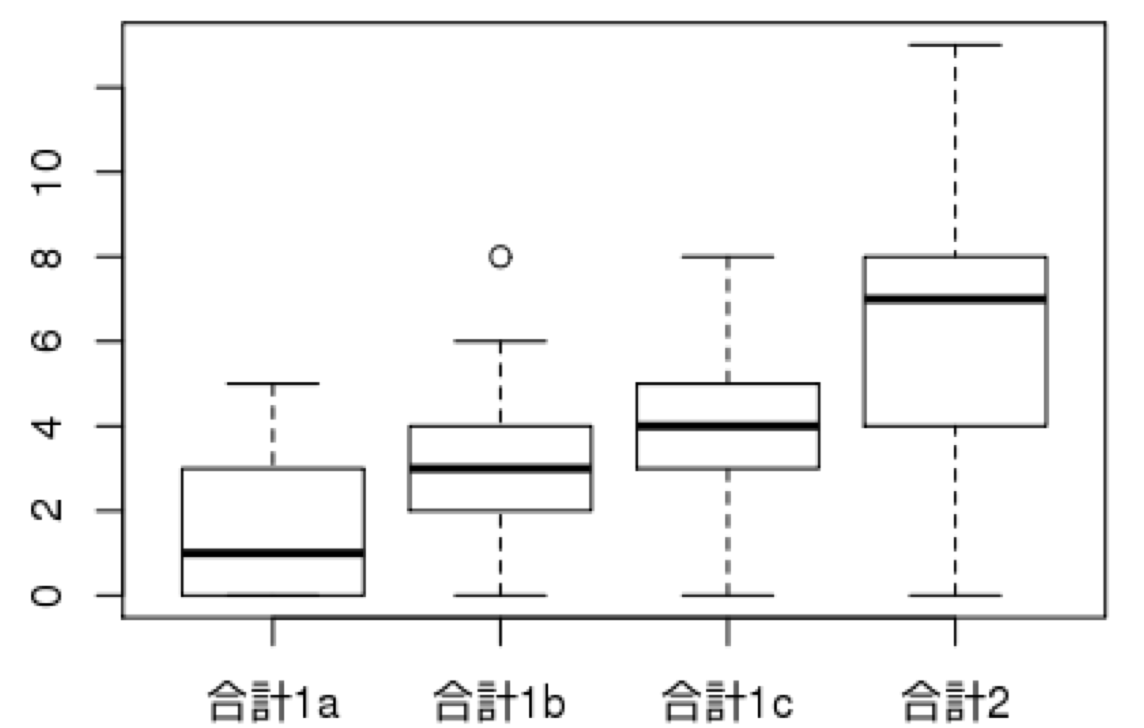
\includegraphics[width=10cm]{./image/D-3-Fig10.png}
  \caption{参加者あたりのテスト条件特定数}
  \label{fig:D-3-Fig10}
  \end{center}
   \end{figure}

今回のワークショップでは, e1a の演習にて,解答をこれまでの経験に基づいて自由に書いてもらうようにした.この結果, テストの記載パターンが4 つに分類できることがわかった.
%<表3 テスト記述パターン>
% Table generated by Excel2LaTeX from sheet 'Sheet4'
\begin{table}[htbp]
  \centering
  \caption{テスト記述パターン}
    \begin{tabular}{|c|p{8.57em}|p{10.215em}|p{3.855em}|}
    \hline
          & \textbf{パターン} & \textbf{記載内容} & \multicolumn{1}{c|}{} \bigstrut\\
    \hline
    1     & 仕様項目  & 「○○な場合に××なること」といったテスト対象の仕様 & 分析的 \bigstrut\\
    \hline
    2     & テストケース & 入力値,アクション,期待結果 & 実装的 \bigstrut\\
    \hline
    3     & P-V
(パラメータ/値) & パラメータと値 & 分析的 \bigstrut[t]\\
    4     & シナリオ  & 操作手順として記載 & 実装的 \bigstrut[b]\\
    \hline
    \end{tabular}%
  \label{tbl:D-3-tbl11}%
\end{table}%

表~\ref{tbl:D-3-tbl11}の1 と3 は中間成果物的であり, 記載した内容を見てそのままテストを実行するには不向きである.
一方,2と4 はそのままテスト実行時に利用できる.
一方, 分析や設計をすると1 と3 が成果物になる.
自由に記載してもらう際に分析結果から書くことは,普段の業務でも分析や設計をしていると想定できる.
なので, 2と4 を直接書くのは, 普段の業務であまり分析や設計行為をしていないのではないかという仮説を持った.
仮説が正しければ, 普段から業務にて分析や設計をしている参加者のほうが, 慣れているために知識の習得が早いと想定し, 今回のワークショップを通じた演習結果にてこれまでの記載方法と演習の成果に相関があるかを調査した.
図~\ref{fig:D-3-Fig13} がスピアマンの順序相関分析をした結果である,
e1a では, 仕様項目から記載する参加者と特定できたテスト条件数には, 0.51(0.4 以上の値は相関ありといえる)の相関が出たたがそれ以外は0.4 以上の値は出なかった. グラフの傾向からは, e2では分析的な記述をしていた参加者のほうが実装的な記述をした参加者より正の相関となったが, 分析結果の値は0.2 をきっているため,相関があるとは結論付けられない.
\begin{figure}[h]
  \begin{center}
  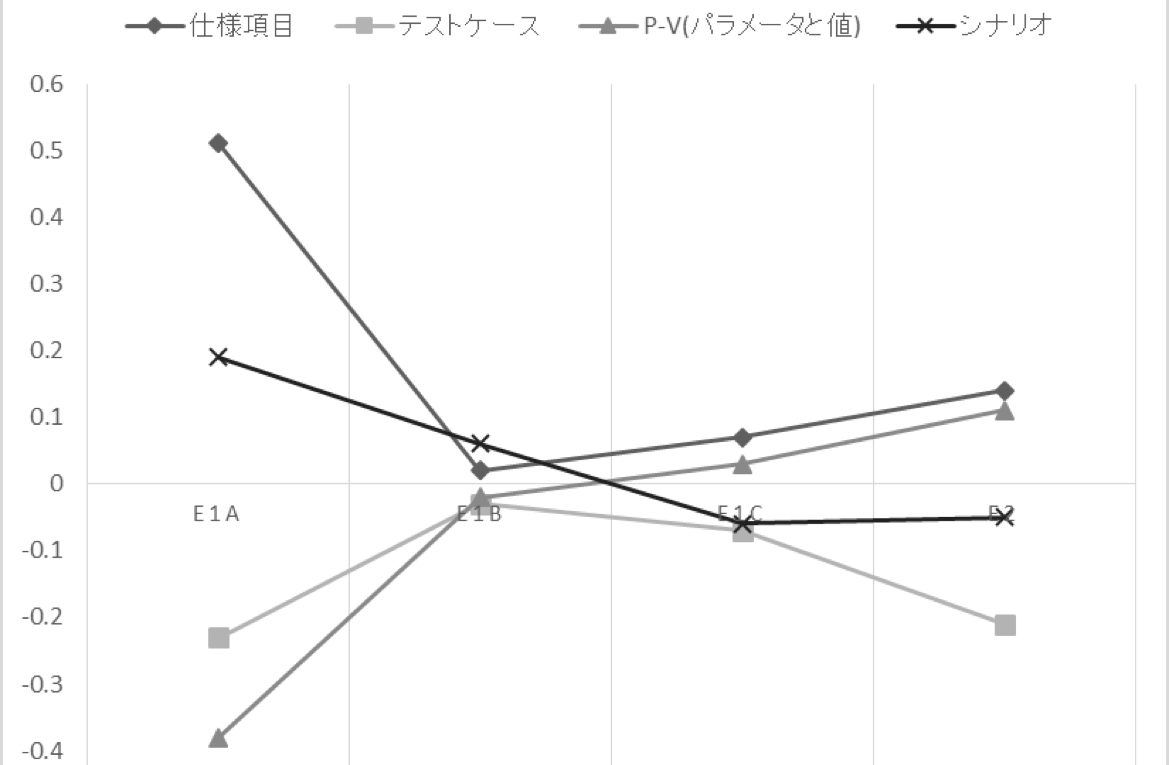
\includegraphics[width=10cm]{./image/D-3-Fig13.png}
  \caption{e1aの参加者業務分野別テスト条件特定数}
  \label{fig:D-3-Fig13}
  \end{center}
   \end{figure}

%The correlation only participants came out to the specifications items of e1a, the test conditions to be specified in this exercise, because it is a specification item itself, the correlation of the the participants result the specifications items in the first exercise It is considered to have moved out.
e1a の仕様項目を記載する参加者だけ相関が出たのは,今回の演習で特定するテスト条件が仕様項目そのものであるため, 最初の演習では仕様項目を記載した参加者と結果の相関が出たと考えられる.

\section{終わりに}
これらの検証実験にて,本手法の説明を参加者にすることによる仕様項目の一貫性と特定する量の向上が観察できた.更にI/Oデータパターンを使った実験結果の分析によって,実験結果の一部が本手法で提唱している仮説と一致することを観察できた.更に高精度に傾向を分析するため,更なる検証実験は必要である.以降のこの手法の効果と関連する要因とその傾向に対する深い理解とそのための更なる実験をすることで,AUTとフォールトの知識をベースにしたテストカテゴリを作るためのルールをより洗練できると考えている.

%%%%%%%%%%%%%%%%%%%%%%%InSTA2015の論文
\chapter{I/Oテストデータパターンを使ったテストケースの特定方法}
\section{既出のテスト分析手法の課題}
これまでの研究では,同一組織内で本手法を導入したグループと導入していないグループでの仕様項目の選択数を比較する実験[4]と,複数のグループに対して本手法の習得前と習得後で選択した仕様項目の数を比較する実験[5]を行った.
どちらの実験でも一貫性のあるルールを適用することでテストケース作成に必要な仕様項目の特定の際に抜け漏れが少なくなることを確認している.しかしながら,今までの研究にて提案した手法は,テストベースの分析に論理的機能構造をガイドとして使用することを明示しているだけであり,具体的な分析手順について定義できていない.
そのため,実験の際に被験者に対して,テスト分析にて仕様項目の選択を網羅的に行う具体的な方法を明確に提示できていない.
本研究では,テスト実行時のデータのI/O に着目した.
テスト実行時のデータのI/Oのパターンを分析の分類に対する全体集合として定義する.テストベースを分析する際にテスト実行時のデータI/Oの要素で分解し網羅性を確認する方法を,既存の手法に追加する.

%\section{An approuch to detarmin spec-item by I/O Test Data Pattarns}
\section{I/Oテストデータパターンを使った仕様項目特定の方法}

\subsection{I/Oテストデータパターン}

テストを実行するためには,データをAUTにインプットし,AUTのアウトプットを期待結果と実際の結果で比較する.
たとえば,シンプルな機能の四則演算の計算結果が正しいことを検証するときには, AUTの外部から複数の値を入力し, AUTがそれらの値を計算し,計算結果をAUTの外部にアウトプットする.これは,図〜ref {fig:D-4-Fig5}で示している例「 Data-in from outside,Data-out to outside,」となる
固定比率が計算結果に適用されるとき(他の計算も適用されると言う意味で),AUTは適切な比率を呼び出し,利用してから計算結果をアウトプットするこれは図〜ref {fig:D-4-Fig5}で示している例「Data-in from outside and inside, Data-out to outside」となる
 \begin{figure}[htbp]
  \begin{center}
  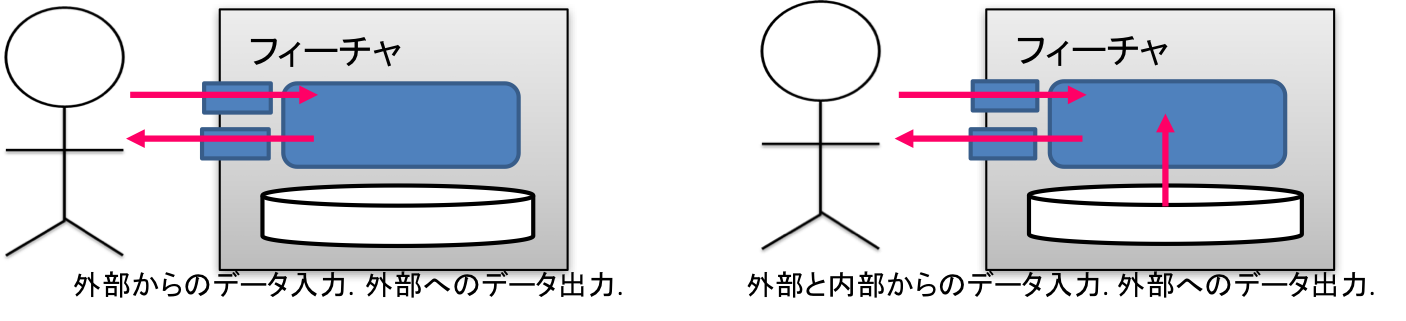
\includegraphics[width=10cm]{./image/D-3-Fig4.png}
  \caption{AUTのデータの入出力の説明}
  \label{fig:D-4-Fig5}
  \end{center}
   \end{figure}


% 注意すべきこととしてI/OデータパターンはAUTの外部からの観察が可能なものを選ぶことがあげられる.処理の起動終了に使われる内部のコマンド(シグナルやイベント)は,データパターンへ分類をするときに考慮しない.なぜならこの手法はブラックボックステストのためのテストベースの分析手法であり,AUT内部のシグナルやイベントのような内部コマンド はブラックボックステストでは,明示的に考慮しないからである.

AUTへのデータの入力の方法は3パターンに分類できる.同じようにAUTからのアウトプット方法は3パターンに集約できる.そのため,AUTに対するテスト実行時のデータの入出力をまとめたパターンは図〜ref {fig:D-4-Fig6}のように9パターンに集約できる.
    \begin{figure}[htbp]
  \begin{center}
  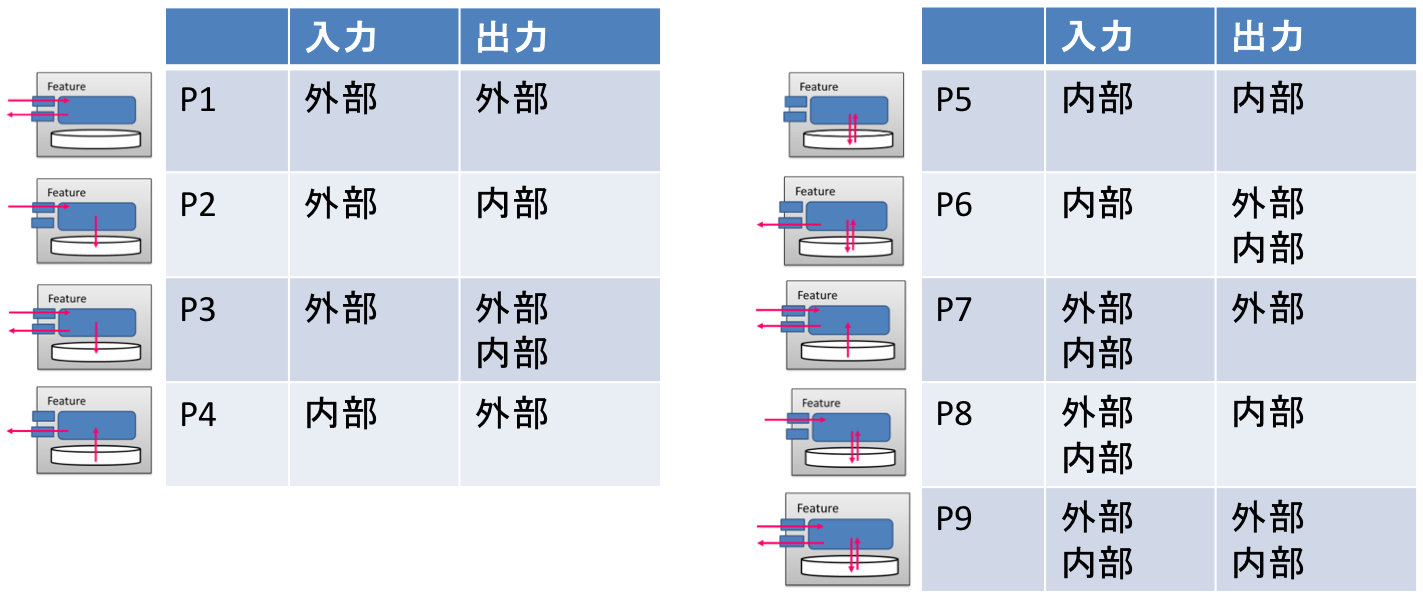
\includegraphics[width=10cm]{./image/D-3-Fig5.png}
  \caption{I/Oデータパターンの説明}
  \label{fig:D-4-Fig6}
  \end{center}
   \end{figure}

これをI/Oテストデータパターンと呼ぶ.
I/Oテストデータパターンがテスト実行時のデータの入出力から見た全体集合となる.
テスト分析のアウトプットである仕様項目は最終的に全て実行して確認することができなければならないので,全てが9パターンのどれかに分類できる.I/Oテストデータパターンと論理的機能構造の要素を対比させて,各パターンがどの要素に該当するかを図\ref{tbl:D-4-tbl1}にまとめた.

%TABLE II. I/O DATA PATTERNS AND THE LOGICAL STRUCTURE OF A FEATURE   \label{tbl:D-4-tbl2}%

たとえば,P1に分類できるシンプルな四則演算の場合,外部からの入力に対して外部に出力する間に,図〜ref {fig:D-4-Fig7}のように論理的機能構造のInput Adjustment,Output Adjustment,Conversionを通過する.そのため,P1はTableIIの3箇所にプロットされている

   \begin{figure}[htbp]
  \begin{center}
  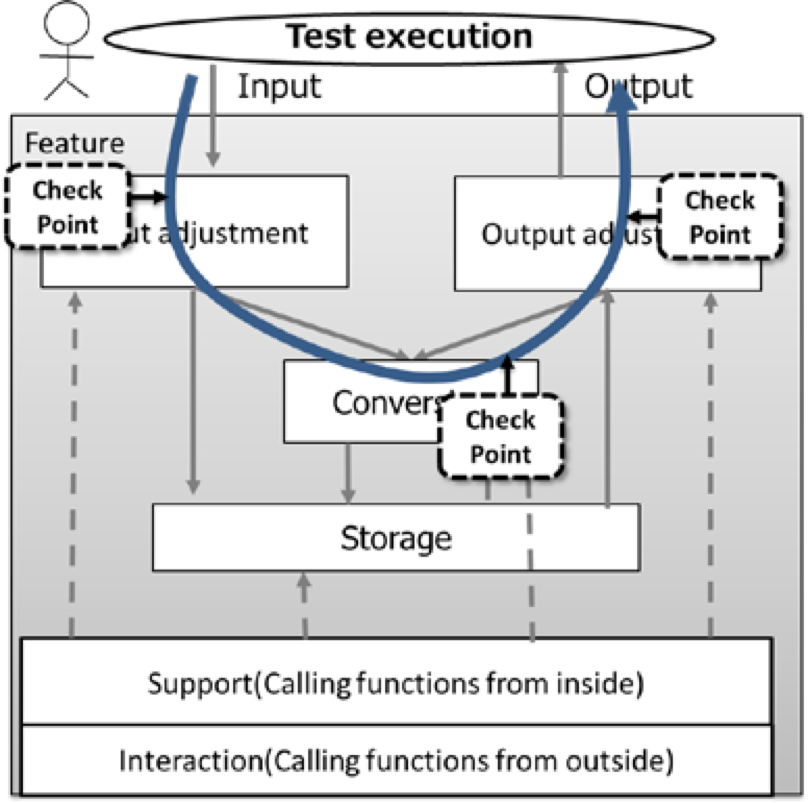
\includegraphics[width=10cm]{./image/D-4-Fig7.png}
  \caption{Fig. 7. An explanation of the I/O data patterns.}
  \label{fig:D-4-Fig7}
  \end{center}
   \end{figure}

しかし,実際に期待結果を確認するチェックポイントは3箇所とは限らない.なぜなら,入力調整に該当する入力の際に適切な値だけ受け入れることと,変換に該当する計算が適切に行われていることの2つだけであり,出力が適切にされることはチェックポイントとしないといったケースが考えられるためである.
 また,TableIII図〜ref {tbl:D-4-tbl1}では,サポートと相互作用についてはデータパターンがプロットされていない.なぜならP1からP9のI/Oデータパターンは単一の入出力の全体像だからである.

%TABLE III. RESULTS FROM EXPERIMENTS PERFORMED IN PREVIOUS STUDIES

論理的機能構造の要素であるInput Adjustment,Output Adjustment,Conversion,Storageは,外部観察可能な単一の入出力のみを考慮している分類であるのに対して,SupportとInteractionは,単一の入出力だけではなく,関係する他の処理の呼び出しに着目して仕様項目を特定するための分類である.
SupportとInteractionに分類される仕様項目は,呼び出した後の出力で期待結果を確認する. 呼び出された機能のI/Oテストデータパターンは,論理的に全パターンが発生する可能性がある.そこで,これまでの研究で行った被験者を使ってテストカテゴリを使った分析手法の習得前と習得後を比較する実験にて使用したテスト分析の講師解答例を同じフォーマットの表に当てはめて,実際の傾向を調査した

\subsection{これまでの実験データを使った調査}
この実験では,ヘッドセットのフィーチャであるボリュームコントロールと,フライト予約システムのフィーチャである新規フライト予約の2種類の異なったAUTを実験に使用した.実験で解答例として作成したテスト分析結果をI/Oテストデータパターンで整理した結果がTableIIIである.この結果からわかるとおり,実際に現れたパターンは,P1とP2 とP4とP7だけであり,P1からP9のパターンの全てが現れなかった.またP1でプロットされているのはInput AdjustmentとConversionのみであり,Output Adjustmentに該当する仕様項目は無かった.同様にP2はStorageのみ,P4はConversionとOutput Adjustmentのみであり,各I/Oデータパターンのデータのフローの中で期待結果を確認するチェックポイントが限られていることが確認できた.

\subsection{サポートと相互作用に関する考察}
また,TableIIでは,SupportとInteractionに分類できるI/Oテストデータパターンを特定できていなかったが,実際のテスト分析結果から調査した結果,
TableIIIで示したとおり,P1とP2とP4とP7に仕様項目を分類できた
TableIVには,TableIIIと同実験にてSupportとInteractionに分類した仕様項目を列挙した.

SupportとInteractionとして特定して仕様項目の傾向について以下のような考察が出来る

Supportは,テスト対象フィーチャでのテスト実行時のアクションによって内部的に呼び出される別の処理の結果確認のことを指している.この例では,全てテスト対象の入力に対して結果を返すだけであるため,I/OテストデータパターンはP1としている


一方,Interactionは,テスト実行時のアクションによる副作用を,他フィーチャに対するアクションにて呼び出して確認することを指している

この例では,ボリュームコントロールの2つの仕様項目は,副作用を確認する際に,該当する他フィーチャにてテスト実行時に外部から入力を与えて結果を確認するためP1にしている.

フライト予約システムの場合は,新規フライト予約にて登録した新規予約が反映していることを他のフィーチャにて確認することを指しているが,テスト実行の際は該当のフィーチャに対して外部入力を与えずともすでに保存された結果の出力で確認ができるためP4としている.

TableVには,各仕様項目を特定する際のきっかけとなる呼び出し方法を列挙した.サポートに該当する仕様項目の特定に使う呼び出しのきっかけと相互作用に該当する仕様項目の特定に使う呼び出しのきっかけを整理することで,他のAUTに適用する際に活用できると考えられるためである.呼び出しのきっかけとI/O test data patternの組み合わせはTableVのように整理できた.

\section{I/Oテストデータパターンを使ったテスト分析の実験}
これまでの実験では,被験者の学習過程に対する効果を検証してきた.また,AUTは,実験用に作られた小さなサンプルを利用していた.本論文の実験では,現実のプロジェクトで作られたテストケースと,今回提案するI/Oテストデータパターンを使ったテスト分析結果を比較し,手法の効果を分析する

\subsection{実験の目的}
この実験は以下の目的で行う.

\subsubsection{I/Oテストデータパターンの効果実証}
\begin{itemize}
\item 目的:今回提案しているテストカテゴリにI/Oテストデータパターンを使う手法が,現実のテスト設計と比較して網羅的に仕様項目を特定できることを確認する.
\item 評価方法:現実のテスト設計の結果と,I/Oテストデータパターンを使った分析結果を比較する.
\end{itemize}


\subsection{実験の題材について}
実験対象のAUTは,実在するオンラインのモバイル写真共有アプリケーションを使った.
簡単なサンプルでは出現しないデータパターンもあるため,現実の複雑なアプリケーションを対象にした.
全機能のうち,「アップロード(デバイス上の写真をオンラインサーバへアップロード)」,「グリッドビュー(オンライン上の写真をデバイスにてサムネイルの一覧として閲覧)」という二つのFeatureをテスト対象として選択した.
この二つの機能を選択した理由は,データの内部への投入を行う機能とデータの照会のみ行う機能とで,I/Oテストデータパターンの出現傾向が異なること調査することが出来ると考えたためである.このアプリケーションの開発にて,実際に使われたテストケースと提案する手法で分析した結果を比較する.

\subsection{実験の実施手順}

 The experiments was conducted following steps:


\begin{itemize}
\item Summed up spec-items from test cases in the real project.
\item テスト対象フィーチャで使われる入力データ,出力データを明らかにする
\item I/Oテストデータパターンを付与する
\item 論理的機能構造とI/Oテストデータパターンを使ってテストベースを分析する
\end{itemize}

\subsubsection{実際のプロジェクトでのテストケースを仕様項目ごとに整理する}
 今回の実験で使う成果物には,テストケースのみであり,テスト分析のアウトプットとなる仕様項目のリストはない.テストケースは,入力値や事前条件を組み合わせた複数のインスタンスであるため,今回の実験のためにテスト分析でのアウトプットである仕様項目と期待結果としてまとめなおす必要がある.図〜ref {fig:D-4-Fig8}のように,テストケースの要素を整理し,同じアクションを行い,同じ期待結果を確認しているテストケースはひとつの仕様項目としてまとめた.

%Fig. 8. An explanation of summed up a spec-item from test cases.
   \begin{figure}[htbp]
  \begin{center}
  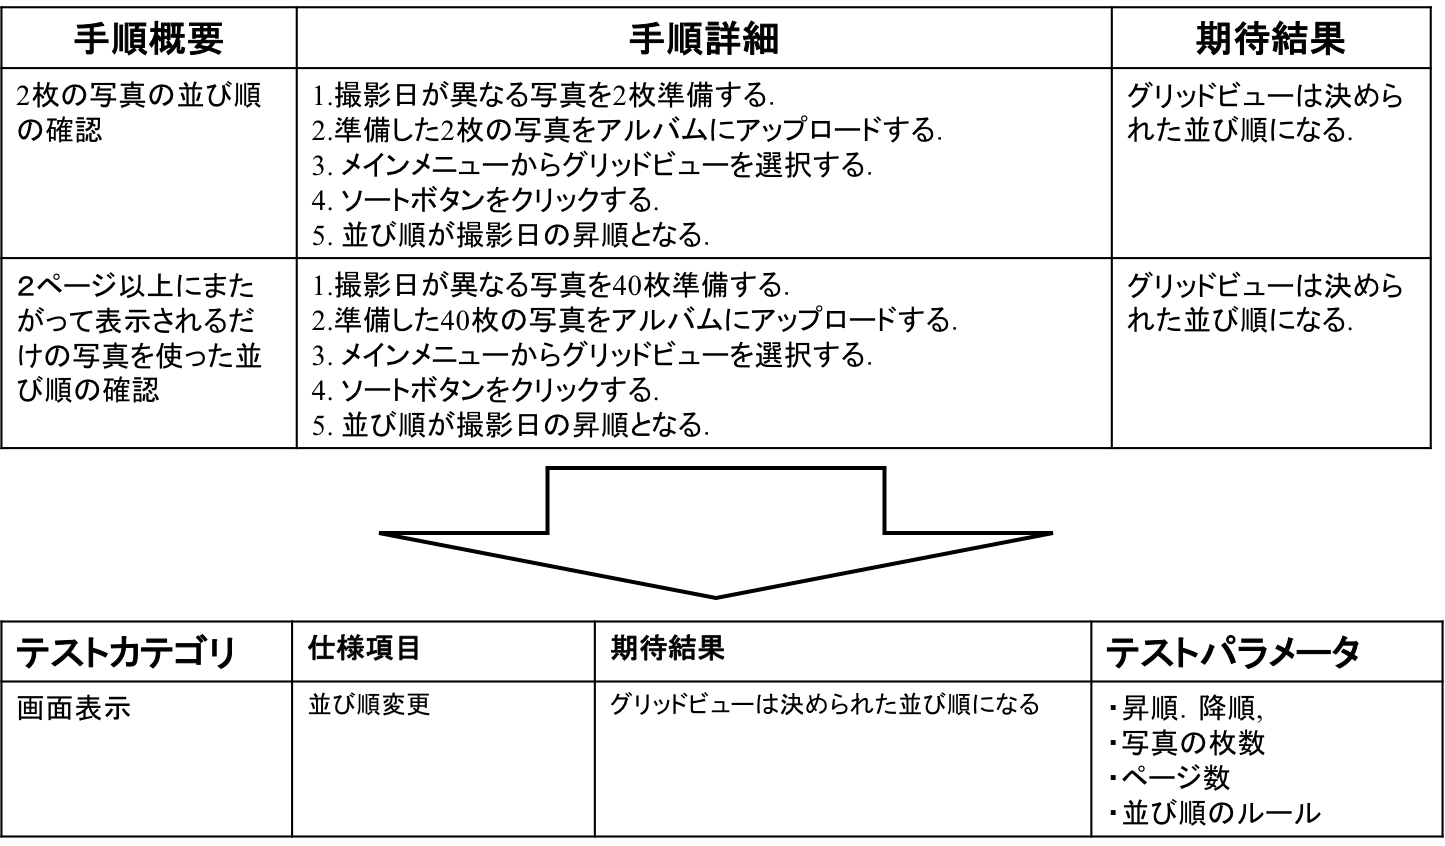
\includegraphics[width=10cm]{./image/D-4-Fig8.png}
  \caption{テストケースから仕様項目をまとめる方法の説明}
  \label{fig:D-4-Fig8}
  \end{center}
   \end{figure}

現場で作られたテストケースの数は,アップロードが491ケース,グリッドビューが151ケースであった.仕様項目として整理した結果,アップロードが59項目,グリッドビューが22項目の仕様項目となった.このように数量が変わる理由は,たとえば「デバイスからサーバーへ画像ファイルをアップロードして保存が出来ること」というひとつの仕様項目に対して,テストケースは,画像の種類(Jpg,Bmpなど),画像のサイズ,アップロードする画像の枚数,画像情報のパターン(ファイル名,撮影日など)といったテストパラメータを組み合わせたものがテストケースとなっているためである.

\subsubsection{2)テスト対象フィーチャで使われる入力データ,出力データを明らかにする}
テスト対象フィーチャであるアップロードとグリッドビューのテストベースを分析し以下の4つを入力データ,出力データとして扱うこととした.
\begin{itemize}
 \item 画像データ
 \item 画像の情報
 \item 設定データ
  \item コマンド
\end{itemize}


\subsubsection{3)I/Oテストデータパターンを付与する}
特定した入力データと出力データは,2)で明らかにした仕様項目に対してFig.9.のリストのようにInput data ,Output dataというカラムに追記していった.テスト実行時の追記したデータの流れをシミュレーションし,該当するI/Oテストデータパターンを明らかにした.図〜ref {fig:D-4-Fig9}は,ソート順の情報を外部から入力し,内部からの入力となる画像データと一緒になり,外部にソートした画像データを表示している例である.この場合のI/OテストデータパターンはP7となる.
%Fig. 9. An explanation of adding input data and output data to a spec item.
   \begin{figure}[htbp]
  \begin{center}
  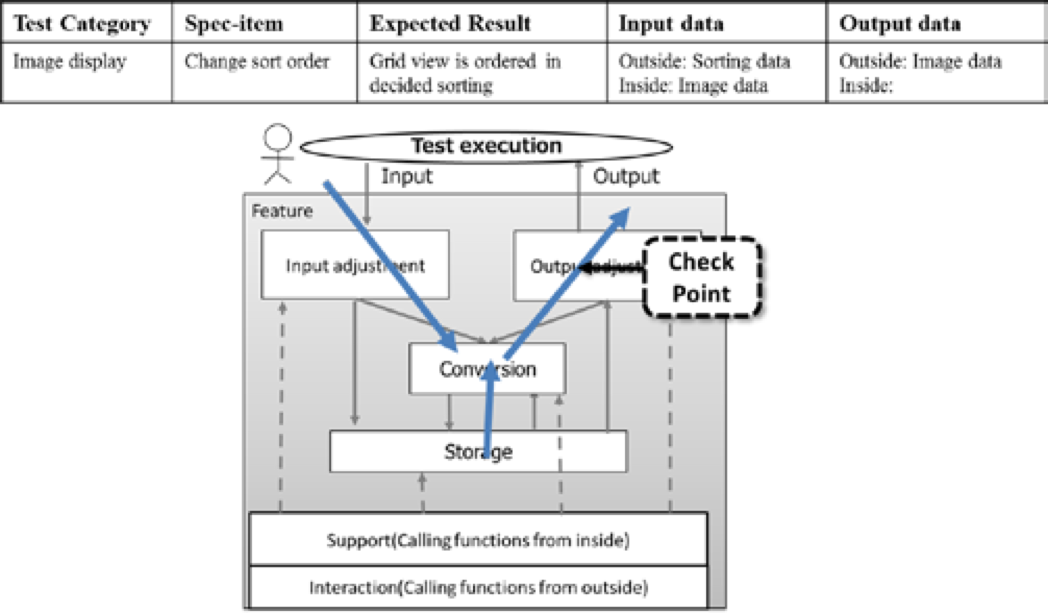
\includegraphics[width=10cm]{./image/D-4-Fig9.png}
  \caption{仕様項目に入力データと出力データを加える方法の説明}
  \label{fig:D-4-Fig9}
  \end{center}
   \end{figure}



\subsubsection{4)論理的機能構造とI/Oテストデータパターンを使ってテストベースを分析する}
I/Oテストデータパターンと既存の分析手法であるテストカテゴリを併用してテスト分析を行う.作業ステップ
は以下のとおりである:

TableVI,VIIのようにテストカテゴリを特定する

テストカテゴリ毎に入力データと出力データを明らかにする

I/Oテストデータパターンごとのデータの流れをシミュレーションして仕様項目を選択する

現場のテストケースを分析した結果をテストカテゴリに分類し,差異を比較する.

SupportとInteractionについては,テストカテゴリとして特定したTriggerで呼び出す機能から仕様項目を選択した

\subsection{実験結果の評価}

\subsubsection{1)IOテストデータパターンの効果実証の結果}
 
テストカテゴリとI/Oテストデータパターンを使ったテストベースの分析を行った結果をTableViiiにまとめた

今回のテスト対象フィーチャであるUploadとGrandviewの 両方でテストカテゴリとI/Oテストデータパターンを使ったテストベースの分析が適用できた.そして,両方のフィーチャにて,現実のAUTに おけるテスト設計と比較し,現場のテスト設計に仕様項目が不足していることが実証できた.分類に利用したI/Oテストデータパターンは,P5とP8を除く全てであった.



実プロジェクトの仕様項目との比較をした結果を図〜ref {fig:D-4-Fig10}に示す.両者を比較すると,テストカテゴリとI/Oテストデータパターンを利用したテスト分析の結果が実プロジェクトより多くの仕様項目を選択できたことが確認できている.
%Fig. 10. Finding the remainder of each data pattarn between Test-Category and the real project.
   \begin{figure}[htbp]
  \begin{center}
  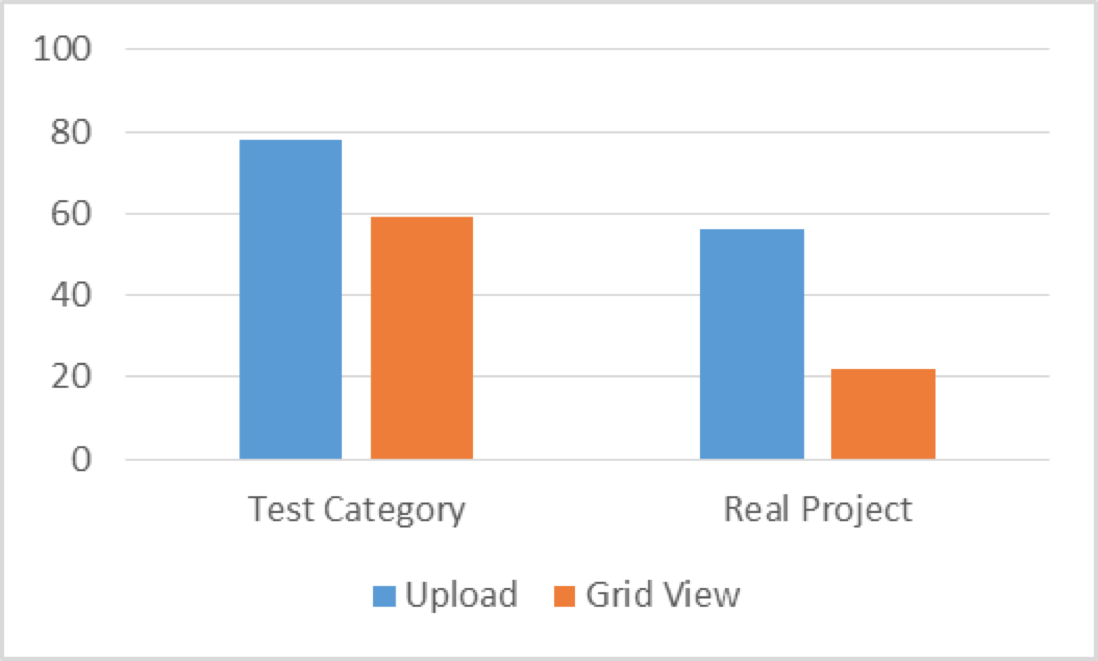
\includegraphics[width=10cm]{./image/D-4-Fig10.png}
  \caption{Finding the remainder of each data pattebrn between Test-Category and the real project.}
  \label{fig:D-4-Fig10}
  \end{center}
   \end{figure}

\subsubsection{2)I/Oテストデータパターン毎の出現傾向の評価}

現実のプロジェクトで作られたテストケースとテストカテゴリとI/Oテストデータパターンを使ったテストベースの分析結果をP1からP9の分類で出現割合を比較した結果が,Table IX.である.それぞれのI/Oテストデータパターンの選択数の差異を図〜ref {fig:D-4-Fig11}にて確認すると,P1が特にテストカテゴリと実プロジェクトの差異が大きいことがわかる.P1は外部からの入力を行い,外部に出力する最も単純なパターンであり,単純なパターンの仕様項目がより網羅的に特定できていたことが確認できる.
%Fig. 11. Finding the remainder of each data pattebrn between Test-Category and the real project.
   \begin{figure}[htbp]
  \begin{center}
  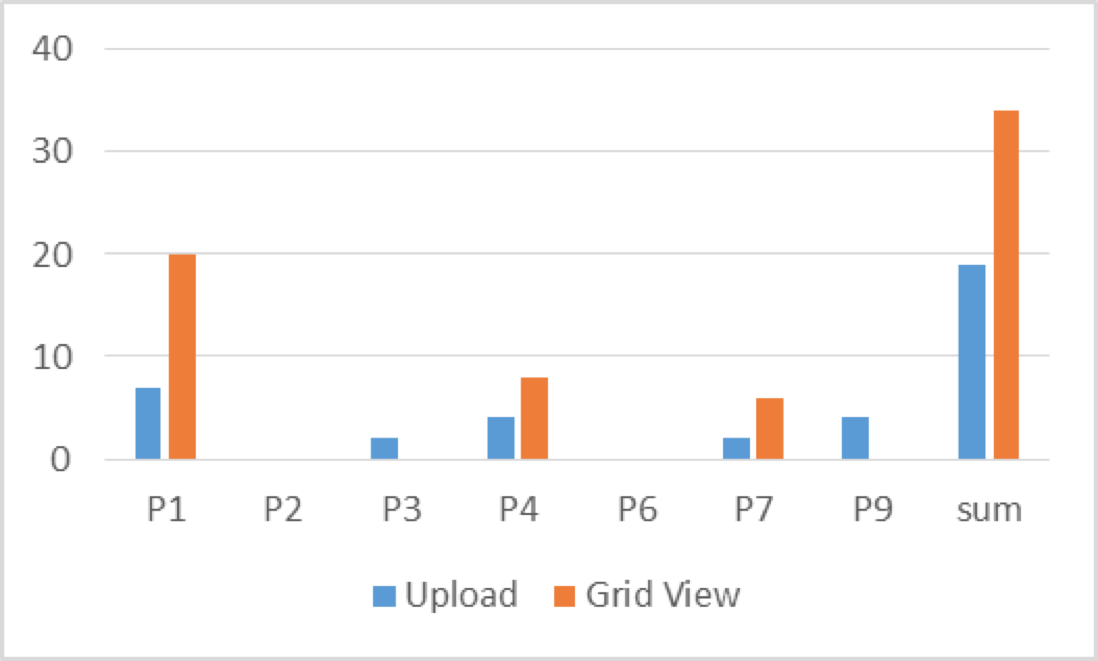
\includegraphics[width=10cm]{./image/D-4-Fig11.png}
  \caption{IOテストデータパターンごとの違い}
  \label{fig:D-4-Fig11}
  \end{center}
   \end{figure}


\subsubsection{3)現実のプロジェクトにて不足していた仕様項目}

TableXには,現実のプロジェクトにて不足していた仕様項目をいくつか抜粋して列挙した.これらの仕様項目は,全て今回のデータのI/Oのシミュレーションを行い網羅的にテストベースを確認することで特定できたものである.不足していた仕様項目には,論理的機能構造の要素別に見てもInput Adjustment, Output Adjustmentといった

メッセージが現れることや入力制御といった単純なことを確認する仕様項目でも漏れているものもあることが確認できる.一般的に,仕様項目のリストを作成せずにテストケースを作った場合,テストケースのままでは数量の多さから網羅すべき仕様項目の見易さが低下するため,仕様項目の数が不足することが多い.実験結果も同様の傾向となった.

\section{終わりに}
 本論文では,テスト実行時のデータI/Oの要素で分類し網羅的に分析する方法を提案した.そして,現場のテストプロジェクトのテストケースを使い,提案した方法の実証を試みた.結果的に,提案した方法で特定した仕様項目と実プロジェクトで作られるテストケースと比較して,不足している仕様項目の発見が可能であることが確認できた.I/Oテストデータパターンを活用したテスト分析をするためには,まだ多くのサンプルを入手し,全てのI/Oテストデータパターンをナレッジにする必要がある.ナレッジにすることで,テスト分析にて仕様項目を効率よく特定するルールを確立させていきたい.

\section{謝辞}
We would like to thank NPO ASTER to use test cases in the real project for the experiment and for allowing us to publish these results.



%%%%%%%%%%%%%%%%%%%%%%%
%電気学会の論文とSSを参考に。現在は変更における状態を含むテスト網羅尺度とテストケース抽出法の提案をコピー
\chapter{データ共有タスク間の順序組合せテストケース抽出手法}

%%%%%%%%%%%%%%%%%%%%%%%
\section{はじめに}
ソフトウェアの一部に変更を加えた場合,その変更の波及を探る変更波及解析(Change Impact Analysis)は,実務上の大きな課題である.
産業界において変更にかかる活動は,新規開発よりも大きな割合を占めている.
ゼロから新規にソフトウェアを開発するケースは稀であり,何らかの流用を基に変更を加える開発が主流となっている.
開発方法においてもアジャイルが主流となり,変更の積み重ねによって開発が行われている.

しかし,変更波及を合理的に制御する技術は,ソフトウェア工学とって未完成の分野である\cite{arnold1996software}.
変更の背景は,時代と共に課題を難しくしている.
ソフトウェアの多様化と複雑化,再利用範囲の増大などから変更波及の範囲が拡大し,かつ安易な変更による弊害など課題が山積している.
これらの課題に対してソフトウェア工学は十分な解を提供できていない状況にある\cite{li2013survey}.


本論文では,状態遷移を持つソフトウェアにおいて,変更波及がデータベースや外部変数などの保持データを介して生ずる場合のテストについて考える.
課題の一つは,網羅基準である.データフローテストの全使用法(AU法)\cite{beiz90}を基にして,変更波及のテスト網羅基準を波及全使用法(Impact Data All Used:IDAU)として提案する.
もう一つの課題は,IDAU法を満たす具体的な変更波及のテストケースの抽出方法である.変更波及のテストの設計手法として,順序組合せテストを提案する.
最後に,ここで提案するIDAU法のコストの評価、すなわちテストケースの数を従来技法である状態遷移テストのS1網羅基準と比較をして考察を行い,提案する方法が合理的であることを示す.

%2 章にて,提案手法の前提となるソフトウェアの構成と変更について定義をし,変更波及のテストの課題について述べる.
%3 章にて,提案手法で用いるルールと,そのルールを適用してテストケースを得るために必要な情報について述べる.
%4 章にて,具体的な例を使って3章で示した手法の適用を確認した.
%5 章にて,従来技法である状態遷移テストのS1 網羅基準と比較をして考察を行った.
%その結果,従来方法であるS1 基準網羅では28 の組合せが抽出されるのに対し,提案手法では5つとなった.


\section{変更波及とその解析}
本節では,提案する網羅基準やテスト設計手法の前提となる,システムの構成と変更について定義し,変更波及テストの課題について詳細を示す.

%−−−-図1を入れる
\begin{figure}[t]
  \begin{center}
  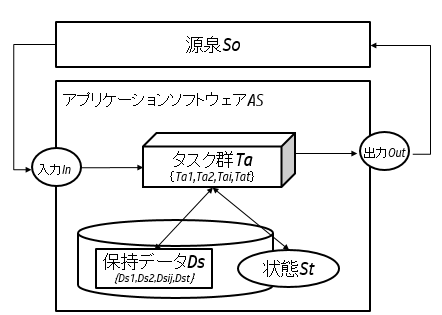
\includegraphics[width=6cm]{./image/fig-1.png}
  \caption{アプリケーションソフトウェアの構成}
  \label{fig:fig-1}
  \end{center}
\end{figure}

\subsection{対象とするアプリケーションの構成}
一般的にソフトウェアは,入力$In$に対して,何らかの出力$Out$を返す.
ソフトウェアの機能は,何らかの入力を出力に変換する処理により実現されていると考えられる.
この処理を本論文ではタスクと呼ぶ.
タスクは,該当のテストレベルからみた入力を出力に変換している1処理である.
そのため,タスクの粒度は,テストレベルによって決まる.%1-3対応
ソフトウェアの構成要素であるタスク$Ta$の出力について考えると,$Ta$への入力$In$だけでなく状態$St$と保持データ(データベースや内部メモリに保存されているデータ)$Ds$の影響を受けると考えられる.
例えば,Webアプリケーションにて予約を行うタスクについて考えると,予約が可能か否かを示す状態と,予約オブジェクトの予約状況を示す保持データによって,予約の成否が決まる.

本論文では,対象として図\ref{fig:fig-1}に示すような状態と保持データを持つアプリケーションソフトウェア($AS$)について考える.
$AS$の構成要素は,タスク群$Ta$と状態$St$と保持データ$Ds$とし,各タスクは外部の源泉$So$からの入力$In$と$So$への出力$Out$があるとする.
タスク群$Ta$は,その要素を$Ta=\{Ta_1,Ta_2,\cdots,Ta_i,\cdots,Ta_t \}$とし,変更タスクを$Ta_i$とする.対応する入出力は$In_i$と$Out_i$とする.

\subsection{変更と変更波及}
$AS$に対して,何らかの変更を加える場合について考える.
変更には,なんらかの意図があり,$AS$が持つ機能の変更であったり,不具合に対する変更や,性能や保守性の改善のためのリファクタリングであったりする.
本論文では,変更の意図については取り扱わず,$AS$の構成要素(タスク,状態,保持データ)に対する具体的な変更について考える.ただし,テスト実行するためには,タスクを動かすことが必要となる.そのため,以降の議論はタスクに焦点を絞る.%1-1対応

ひとつの変更$Q$について考える.
変更$Q$は,タスク群$Ta$のあるタスク$Ta_i$に対して行われたとする.
変更$Q$は,コードの削除や追加を含み,その結果$Ta_i$の版$R$が$R+1$に変更される.
この変更の結果を$Ta^{R}_i$から$Ta^{R+1}_i$とする.

変更$Q$の波及には,3つのケースが考えられる.
\begin{enumerate}
  \item 変更波及が無い場合.(リファクタリングに相当)
  \item 変更波及が他のタスクへ波及しない場合.%3-7対応
  \item 変更波及が他のタスクへ波及する場合.
\end{enumerate}

3.の変更波及は,タスク間の参照が図\ref{fig:fig-2}に示すように状態と保持データに限られるならば,該当する状態や保持データの参照を介した範囲が限られると考えられる.
本論文では,この考え方から波及を受けるタスクを特定し,その合理的なテスト設計について論じる.


%−−−-図2を入れる

\begin{figure}[b]
\begin{center}
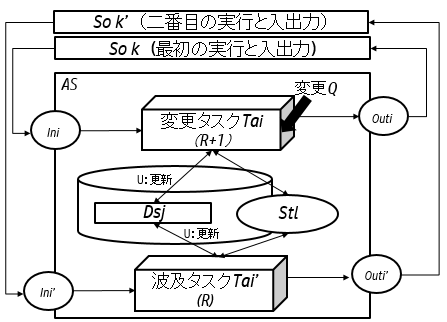
\includegraphics[scale=0.5]{./image/fig-2.png}
\end{center}
\caption{変更タスクと変更波及}
\label{fig:fig-2}
\end{figure}

変更波及,あるいはその解析(Change Impact Analysis)に関する研究は古くから行われている.プロダクトラインやUML図面群を基に依存関係生成モデルを用いて波及解析を行う研究がある\cite{gomaa2005designing,briand2003impact,小谷正行2008}.
タスク内のデータフローを基に変更波及を詳細に解析した研究がある\cite{campbell1990}.
データベースなど保有データを基に変更波及解析を行う研究も行われている\cite{maule2008impact,加藤正恭2011}.
一方,状態と状態遷移はマルコフ過程として実装されているので,過去の状態が未来の状態に影響しない.状態遷移に関する波及解析の研究は見当たらないのはそのためだと推測する.%3-8対応

\subsection{状態と変更波及のテスト}
変更波及は,保持データを介して波及タスクへ伝達する.状態や状態遷移自身は変更波及に関与しないが,変更波及のテストにおいて与えるデータの順序において状態を考慮する必要が生じる.

保持データの構成について考える.その要素を$Ds=\{Ds_1,Ds_2,\cdots,Ds_j,\cdots,Ds_d\}$とし,変更波及を受ける保持データの要素を$Ds_j$とする.
保持データに対する操作は,データのライフサイクルである「生成:C」「参照:R」「更新:U」「削除:D」を記したCRUD図で定義する.
$Ds_j$を介して変更波及が生ずるのは,変更タスク$Ta_i$において「生成:C」あるいは「更新:U」が行われ,他のタスクで「参照:R」が行われた場合に波及タスクとなる.

保持データのライフサイクル上の「生成:C」「参照:R」「更新:U」「削除:D」などの操作は,無条件に行われるのではなく,操作するタスクの制御フローに沿って行われる.
制御フローは,2階層として捉えることができる.上位の制御フローはタスクの実行順序により決定される大きな制御の流れに相当する.
個々のタスク内の制御フローが下位にあたる.個々のデータ参照実行文はその制御フロー上の条件文で実行が決定される.
条件にはタスクへの入力,保持データ,状態が含まれる.

変更波及を確認するには,変更が波及した保持データを参照するデータフローに沿ってテストを設計することになる.
このデータフローを決定するのは,関係するタスクの実行順序とタスク内の制御フローであり,その制御フローを決定する際に状態が影響する.
状態による制御が想定通りに行われない欠陥は,タスクの実行順序により決定される大きな制御の流れの判断のための状態の確認を,タスク実行のあるタイミングでのみ行っていることが原因となる.%1-2対応による追記
よって,実際のテスト実行においては状態を考慮する必要が生ずる.

\subsection{変更波及テストの網羅基準}

テストにおける網羅基準については,その強度を含め制御フローとデータフローの観点から研究が行われ体系が作られている\cite{beiz90}.
最も弱い網羅基準は制御フローのみに着目した実行文網羅,次が分岐網羅であり,最も強い網羅基準はデータフローを含めた全パス網羅(All Paths)である.%3-9
全パステストは,すべての分岐の積であり現実的には実現不可能のため,全使用法(All Uses)が推奨されている\cite{beiz90}.

変更波及をテストする場合,波及に関与するデータに着目し,そのデータフローテストを行う.
一般的な全使用法は「データを定義したすべての場所から始まり,データを使用するすべての場所に至るまでのパスセグメントを最低限1つを含むテストケース」と定義されている\cite{beiz90}.
%この定義を変更タスクと波及タスクとの関係に置き換え「変更タスクにおいてデータの定義,あるいは更新があるデータについて,そのデータを使用する全てのタスクはタスク経路にかかわらず最低限1つを選択し,タスク内でのすべての使用箇所において最低限1つを含むテストケース」とし,波及全使用法とする.3-10対応
この定義を変更タスクと波及タスクとの関係に置き換え「変更タスクにおいてデータの生成および更新があるデータを使用するすべてのタスク(波及タスク)を2つのタスクを実行するまでに経由するルートにかかわらず最低限1つ含むテストケース」とし,波及全使用法とする.

%-----------------------------------------------
%ここからSS2017用に修正している.湯本
%------------------------------------------------

\section{順序組合せによるテストケース抽出法}

%本章では,変更タスクと波及タスクの実行順序の組合せを抽出する手法として順序組合せテストを提案する.
本節では,図2で示した変更タスクと波及タスクの組合せを抽出する手法として順序組合せテストを提案する.
この手法では,必ず変更タスクを実行した後に波及タスクを実行する,といったように組み合わせるタスクの実行順序を明確にするため,順序組合せと命名した.
\subsection{提案手法に必要となる入力情報}
 一般的にテストケース抽出のために必要な入力情報をテストベースと呼ぶ\cite{Demarco}.
提案手法に必要なテストベースは DFD,ER 図,CRUD 図である.以下,DFD,ER 図,CRUD 図を簡潔に説明する.

\begin{itemize}

\item DFD(データフローダイアグラム)

DFDはシステムにおけるデータの流れを表現した有向グラフであり,要求分析において用いられている.
DFDはデータ指向設計の要として用いられ,オブジェクト指向設計においても抽象化する前段階として実践の場で用いられている.

DFDは,最上位のコンテキストレベルから階層として詳細化され,各階層は1枚以上のDFDから成る\cite{Demarco}.
テストベースとして用いる場合,テストの範囲はDFDで与えられるとする.DFDの階層が下がると単体テストとなり,上がると統合テストとなる.

DFDはノードとエッジからなる.
ノードは3種類の要素である$N$個のタスク(プロセス)$Ta$と,$M$個の保持データ(データストア)$Ds$と,$L$個の源泉(外部エンティティ)$So$から構成されている.%3-11対応
3種類の要素を一意に特定する際は$Ta_i$,$Ds_j$,$So_k$と表記する.

エッジは,ノードからノードへのつながりを有向線分で表記している.エッジはデータの流れを表しており,制御の流れは表していない.
エッジの特定は,起点ノードと終点ノードを用いて行う.
ある特定のタスクからデータストアへの入力がある場合のエッジの特定は,$Ta_i/Ds_j$となり,源泉から出力してタスクで処理をする場合は,$So_k/Ta_i$と表す.%3-12対応

\item ER図

ER図はシステムにおけるエンティティ間の関係を示す図であり,UMLのクラス図に対応している.
DFDでは表現できないエンティティの詳細化やエンティティ間の関係について示しており,DFDと共に用いられている.

ここでは,DFDのデータストア$Ds_j$が持つエンティティと,CRUD図の対応から,後述する拡張CRUD図を作成するために用いる.
よって,テストベースとしては,システムすべてのER図を必要とするものではない.

\item CRUD図

CRUD図とは,タスク$Ta_i$からデータストア$Ds_j$への$C$:生成,$U$:更新,$R$:参照,$Ds$:削除の操作を表した図である\cite{Politano}.
CRUD図から,DFDとER図では表現されていないタスクのエンティティへの操作を知ることができる.

本論文では,タスクがデータストアに対して行う操作を特定するためにCRUD図を用いる.
タスク$Ta_i$のデータストア$Ds_j$に対する操作が$U$:更新であればタスクによる操作はエッジを介した操作として$Ta_i/Ds_jU$と表記する.
ただし,タスクが操作するデータストアが1つだけの場合は,$Ta_iU$といった省略した表記を使う.
\end{itemize}


\subsection{順序組合せテストの概要}
提案する手法は,2タスク間の順序組合せを対象とする.
%データストアを共有しないタスク間の組合せは, マルコフ連鎖を前提として順序組合せテストの対象から除外する.
%データストアを共有していないため,画面遷移あるいは状態遷移は独立しており,S0網羅基準にてテストを行えば十分だと考えられるからである.
2タスク間の順序組合せの抽出は以下のルールを適用する.
\begin{itemize}

\item ルール1:変更タスクの特定
%20170305
%対象とするDFDにおけるタスクにおいて,源泉$So$からの入力エッジがあり,かつデータストア$Ds$へ出力エッジを持つタスクを選択し順序組合せの変更タスク群$P\{Ta\}$とする.

対象とするDFD内の変更タスクのうち,データストア$Ds$へ出力エッジを持つタスクを選択し,順序組合せの変更タスク群$P\{Ta\}$とする.%3-14対応
変更タスク群からの出力するデータストア群を$P\{Ds\}$とする.

\item ルール2:波及タスクの特定
%20170305
%ルール1で求めた$P\{Ds\}$からの入力エッジを持つタスクにおいて,$So$へ出力エッジを持つ波及タスク群$S\{Ta\}$を特定する.

ルール1で求めた$P\{Ds\}$からの入力エッジを持つタスクを波及タスク群$S\{Ta\}$として特定する.

\item ルール3:順序組合せテストケースの抽出

拡張CRUD図を基に変更タスク群$P\{Ta\}$とそのデータストア群$P\{Ds\}$を介する波及タスク群$S\{Ta\}$を組合せ,順序組合せのテストケースとする.
\end{itemize}

以降からは,順序組合せを抽出してテストケースとするまでの実施手順を詳細に説明する.

% Table generated by Excel2LaTeX from sheet 'Sheet1'
\begin{table}[t]
\caption{拡張CRUD図}
\label{CRUDIO}
\begin{center}
\begin{tabular}{r|r|r|r|r|r|r}
\multicolumn{1}{c|}{タスク} & \multicolumn{3}{c|}{データストア} & \multicolumn{3}{c}{源泉} \\
\cline{2-7}\multicolumn{1}{c|}{} & $Ds_1$ & $...$ & $Ds_j$ & $So_1$ & $...$ & $So_k$ \\
\hline
\hline
$Ta_1$ &   &   &   &   &   &  \\
\hline
$...$ &   &   &   &   &   &  \\
\hline
$Ta_i$ &   &   &   &   &   &  \\
    \hline
\end{tabular}%
%\halflineskip
\end{center}
\end{table}

\subsection{ルール1:変更タスクの特定}
ルール1を用いて変更タスクとそのデータストアを特定し,拡張CRUD図の変更タスク部分を作成する.

拡張CRUD図とは,テストベースとして与えられたDFD,ER図,CRUD図から$P\{Ta\}$の各$Ta_i$と関連する$So_k$,そして$P\{Ds\}$となる$Ds_j$の関係を追加して作成したものである.
表 ~\ref{CRUDIO}に拡張CRUD図の表記を示す.
拡張CRUD図のデータストアに対する情報は$C$,$U$,$R$,$D$のいづれか,または組合せか空白である.
源泉に対する情報は$In$か$Out$,または組合せか空白である.
空白は関係が無いことを示す.

\begin{enumerate}
\item 源泉からの入力エッジを持つ変更タスクの特定

%状態について記載するように変更した.補集合で表現するようにした
%元のストーリーである、外部入力があるタスクはそのままにして、更に抽出する要素として、「変更のある」を追加した.
テストケースは,外部からのテスト対象への入力から,外部への出力結果を確認するものであるため,テスト入力とテスト結果のペアで構成されている.
そこで,テスト対象範囲の外からの入力,即ち$So_k$からの入力エッジを持つ$Ta_i$を見つける必要がある.
この特性を持ったタスクのうち,さらに変更のあるタスク群を変更タスクの集合となる$P\{Ta\}$候補とする.
変更が特定の状態でのみ起こり得る場合は,タスクの後に変更が起きる状態を[$St_l$]と記載する.
%上記は追加部分

\item データストアへの出力エッジを持つタスク特定

$Ta_i$から$Ds_j$への出力エッジは,$C$か$U$か$D$の操作を行うことを意味する.CRUD図から該当する出力エッジを持つ$Ta_i$を選択する.
$P\{Ts\}$候補の中から,該当する$Ta_i$を選び,変更タスク群$P\{Ta\}$を確定する.

\item 中間の拡張CRUD図作成

拡張CRUD図には,変更タスク群$P\{Ta\}$に該当する$So_k$から$Ta_i$への入力($In$),もしくは$Ta_i$から$So_k$への出力($Out$)の情報を付加する.
特定した$Ta_i$に対して,入力となる$So_k$に$In$を記入し,$Ds_j$についてはCRUD図を参照して$C$か$U$か$D$かその組合せかを記入する.
中間の拡張CRUD図として例示した表 ~\ref{CRUDIO2}では,3つの源泉$\{So_1,So_2,So_3\}$と3つのデータストア$\{Ds_1,Ds_2,Ds_3\}$があり,2つのタスク$\{Ta_1[St_1],Ta_3[St_1]\}$が変更タスクである.
この段階で作成する拡張CRUD図は,作業途中のものである.

\end{enumerate}


% Table generated by Excel2LaTeX from sheet 'Sheet1'
\begin{table}[t]
  \centering
  \caption{中間の拡張CRUD図の例}
    \begin{tabular}{r|r|r|r|r|r|r}
    \multicolumn{1}{c|}{タスク} & \multicolumn{3}{c|}{データストア} & \multicolumn{3}{c}{源泉} \\
\cline{2-7}    \multicolumn{1}{c|}{} & $Ds_1$ & $Ds_2$ & $Ds_3$ & $So_1$ & $So_2$ & $So_3$ \\
    \hline
    \hline
    $Ta_1[St_1]$ & $CU$ &   &   & $In$ &   &  \\
    \hline
    $Ta_3[St_1]$ &   & $C$ &   & $In$ &   &  \\
    \hline
    \end{tabular}%
 \label{CRUDIO2}
\end{table}%

\begin{table}[h]
\caption{タスク間のデータ共有の組合せパターン}
\label{table:3}
\begin{center}
\begin{tabular}{c|c||c|c|c|c}
\hline
\multicolumn{2}{c||}{}& \multicolumn{4}{c}{$P\{Ta\}$}\\
\multicolumn{2}{c||}{}& C & R & U& D\\
\hline\hline
$S\{Ta\}$&C&×&×&×&◯\\
\cline{2-6}
&R&◯&-&◯& -\\
\cline{2-6}
&U&◯&-&◯&×\\
\cline{2-6}
&D&◯&- &◯&×\\
\hline
\end{tabular}
%\halflineskip
\end{center}
\end{table}

% Table generated by Excel2LaTeX from sheet 'Sheet1'
\begin{table}[t]
  \centering
  \caption{完成した拡張CRUD図の例}
    \begin{tabular}{r|r|r|r|r|r|r}
    \multicolumn{1}{c|}{タスク} & \multicolumn{3}{c|}{データストア} & \multicolumn{3}{c}{源泉} \\
\cline{2-7}    \multicolumn{1}{c|}{} & $Ds_1$ & $Ds_2$ & $Ds_3$ & $So_1$ & $So_2$ & $So_3$ \\
    \hline
    \hline
    $Ta_1[St_1]$ & $CU$ &   &   & $In$ &   &  \\
    \hline
    $Ta_3[St_1]$ &   & $C$ &   & $In$ &   &  \\
    \hline
    $Ta_2[St_1]$ & $R$ &   &   &   & $Out$ &  \\
    \hline
    $Ta_5[St_1]$ &   & $R$U &   &   &   & $Out$ \\
    \end{tabular}%
  \label{excrud}%
\end{table}%

\subsection{ルール2:波及タスクの特定}
ルール2を用いて波及タスク群を特定し,拡張CRUD図へ波及タスク部分を追加し図を完成させる.

\begin{enumerate}
\item データストアを介した波及タスク特定
%なぜ\UTF{2613}と−がテストしなくてよいかということを追記した.

先に作成した中間の拡張図から変更タスクの操作が$C$か$U$か$D$であるデータストアに着目する.
着目したデータストアに対してエッジを持つタスクが波及タスクの候補となる.
波及タスクとして選択するタスクは表 ~\ref{table:3}に示す表の○印の組合せに該当するタスクである.
%ここから--ような感じでつじつま合わせたことを松尾谷さんと議論する
%アプリケーション内部での保持データの使われ方がわかっていれば,波及タスクは,R:参照をするものだけでよいが,ブラックボックステストの場合,外部観察で確認をするしかないため,R:参照をした結果利用されていることがわかる処理となる,C:生成,U:更新,D:削除も波及タスクとして選択する.%3-16対応
%ここまで--ような感じでつじつま合わせたことを松尾谷さんと議論する
波及タスクは, C:生成,U:更新,D:削除を選択する.
”-”をつけた組合せは,データストアを介した影響が生じないため,組合せテストの対象としない.
”×”をつけた組合せは仕様上有り得ない組合せであり,ありえないことの確認は,順序組合せを網羅しなくともよいため,組合せテストの対象としない.


\item 拡張CRUD図の完成

波及タスク候補のうち,源泉に出力エッジを持つタスクを波及タスクとして特定する.
波及タスクの特性をDFDより読み取り,特定する.
特定した波及タスクを拡張CRUD図に追記し完成させる.

完成させた拡張CRUD図の例を表~\ref{excrud}に示す.
この例では,
データストア$Ds_1$から源泉$So_2$への流れをタスク$Ta_2[St_1]$が行い,
データストア$Ds_2$から源泉$So_3$への流れをタスク$Ta_5[St_1]$が行っていることを示している.

\end{enumerate}

\subsection{ルール3:順序組合せテストケースの抽出}
拡張CRUD図を基に順序組合せのテストケースを抽出し,テストケース表を作成する.

\begin{enumerate}
\item 変更タスクと波及タスクの組合せを抽出

拡張CRUD図から変更タスクを選ぶ.
先に作成した拡張CRUD図の例(表~\ref{excrud}を参照)であれば,$Ta_1[St_1],Ta_3[St_1]$である.
次に変更タスクが操作しているデータストアと,それを操作している波及タスクを対応付ける.
例では,$Ta_1[St_1]  \xrightarrow[Ds_1]{} Ta_2[St_1]$と$Ta_3[St_1]  \xrightarrow[Ds_2]{}  Ta_5[St_1]$である.


\item データストアに対する操作の組合せ

操作の組合せとは変更タスクと波及タスクの操作の組合せである.
%表 ~\ref{excrud}の例であれば,変更タスクのデータストアに対する操作,$Ta_1$は$Ds_1$に対して$CU$の操作を行っている.%3-21対応
表 ~\ref{excrud}の例であれば,変更タスクのデータストアに対する操作である$Ta_1$は,$Ds_1$に対して$C$と$U$の操作を行っている.
波及タスク$Ta_2$の操作は$R$である.
組合せは$C  \rightarrow R$と$U  \rightarrow R$となる.
変更タスクと波及タスク間に介在するデータストアが1つであれば$\xrightarrow[Ds_1]{}$を省略して$\rightarrow$で表してもよい.
また変更の発生条件となる状態が1つであれは,$[St_1]$を省略してもよい.
表~\ref{excrud}の例における全組合せは,$Ta_1C \rightarrow Ta_2R$,$Ta_1U \rightarrow Ta_2R$,$Ta_3C \rightarrow Ta_2R$,$Ta_3C \rightarrow Ta_2U$の4個である.
%表記上,変更タスクと波及タスクも表すと$Ta_1C  \xrightarrow[Ds_1]{} Ta_2R $,$Ta_1U  \xrightarrow[Ds_1]{} Ta_2R $である.




\item テストケース表の完成

変更タスクと波及タスクの操作の組合せをテストケースとしてまとめる.表 ~\ref{TCLISTSAMPLE}にその例を示す.概要の部分は,当該組合せが持つ入力の条件や出力の特性を仕様から抜き出して記載する.

%--------------------------------

\end{enumerate}

% Table generated by Excel2LaTeX from sheet 'Sheet1'
\begin{table}[t]
  \centering
  \caption{順序組合せテストによる論理的テストケースの例}
    \begin{tabular}{l|l|l}
    No & 論理的テストケース & 順序組合せ \\
    \hline
    1 & 概要 & $Ta_1C \rightarrow Ta_2R$ \\
    \hline
    2 & 概要 & $Ta_1U \rightarrow Ta_2R$ \\
    \hline
    3 & 概要 & $Ta_3C \rightarrow Ta_2R$ \\
    \hline
    4 & 概要 & $Ta_3C \rightarrow Ta_2U$ \\
    \hline
    \end{tabular}%
\label{TCLISTSAMPLE}
\end{table}%



以上の手順で,順序組合せテストに必要なテストケースを抽出する.
ここで用いたテストケースとは,ISTQBの定義による論理的テストケースに相当する\cite{ISTQB}.
%変更した.状態遷移について触れた.
具体的な値や期待結果,該当の処理までの状態を遷移させていく手順まで定義した記述を具体的テストケースと呼ぶが,本論文では扱わない.

\section{順序組合せテストの適用評価}

本節では,旅行代理店向けフライト予約システムの仕様を用いて,3章で述べた実施手順を適用し,順序組合せが抽出できることを確認する.
\subsection{題材の概要}
フライト予約システムの概要を以下に示す.
%・フライト予約システムの概要を説明する\\
\begin{figure}[h]% fig.1
\setbox0\vbox{%
{\scriptsize
%{\footnotesize
\hbox{\verb/<フライト予約システム概要>/}
\hbox{\verb/・旅行代理店用に開発したフライト予約サーバにインターネット経由で/}
\hbox{\verb/ アクセスできる専用のクライアントアプリケーション./}
\hbox{\verb/・旅行代理店の窓口での利用を想定しており,ユーザ認証されたユーザ/}
\hbox{\verb/ のみ利用可能である./}
\hbox{\verb/・旅行代理店の窓口数(クライアント数)は50としており,同時に予約/}
\hbox{\verb/ 処理を行うことができる./}
\hbox{\verb/・旅行代理店にて取り扱う全ての航空会社の飛行機の予約が可能で/}
\hbox{\verb/ ある./}
\hbox{\verb/・本システムは,フライト予約サーバを仲介して複数の航空会社のシス/}
\hbox{\verb/ テムと同期をする./}
\hbox{\verb/・チケット情報や残チケット数は同期することで最新に更新される./}
\hbox{\verb/・フライトの新規予約、予約内容の更新,削除が可能である.更新と/}
\hbox{\verb/ 削除は新規予約したユーザのみ可能である./}
\hbox{\verb/・以下はシステム範囲外/}
\hbox{\verb/ -チケット代金の決済(別システムと連携して行うため)./}
\hbox{\verb/ -マスタ情報設定(他システムとの共用マスタ設定アプリケーションが/}
\hbox{\verb/  あるため)./}
}
}
\begin{center}
\fbox{\box0}
\end{center}
\caption{フライト予約システムの概要}
\label{OVSPEC}
\end{figure}

\begin{figure*}[tb] %ER図とDFD.最初と最後に*を入れると1段で入る
\begin{center}
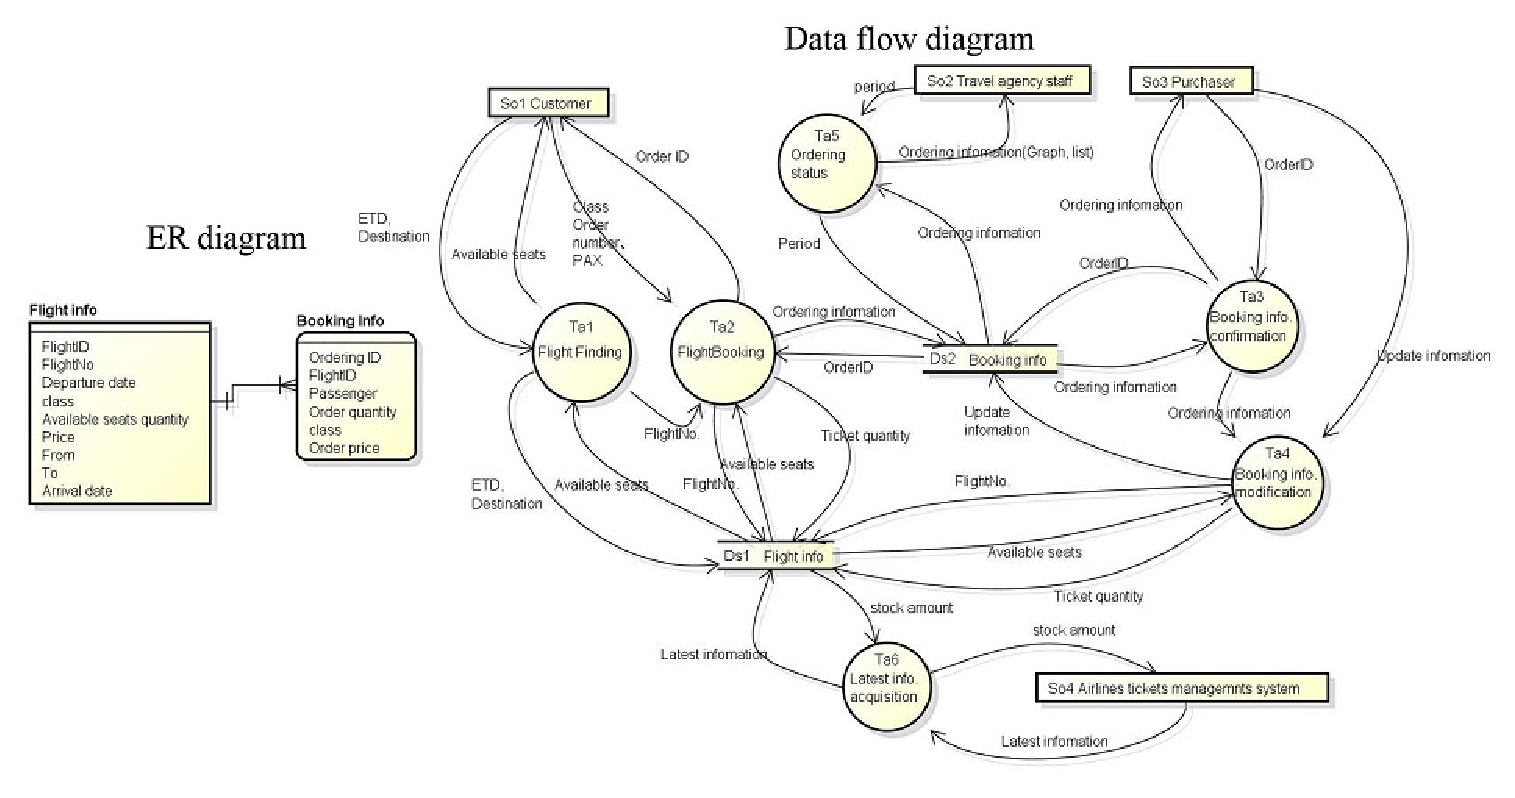
\includegraphics[scale=0.68]{dfdanderd.eps}
\end{center}
\caption{新規フライト予約のデータ設計(一部分)}
\label{fig:DFD}
\end{figure*}

題材となるフライト予約システムの仕様は,本研究の一環として評価実験の際に題材として使っているものである\cite{Yumo2014}.
テスト対象の分析と,テストケース設計に関する用語は,国際標準であるISO/IEC/IEEE29119の定義に従い,テスト対象の論理的なサブセットを機能セット(Feature set)と呼ぶ\cite{29119}.%3-22対応
本論文では,表~\ref{Featurelist}の新規フライト予約を,変更が入った機能セットとする.
新規フライト予約からテストケースを抽出するための前提として用意した仕様は,新規フライト予約に関連するDFDとER図(図~\ref{fig:DFD}),CRUD図(表~\ref{CRUD})とする.
DFDに含まれるタスク数 $N$は6,データストア数$M$は2,源泉数$L$は4である.

\begin{table}[t]
\caption{フライト予約システムの機能セット一覧}
\label{Featurelist}
\begin{center}
\begin{tabular}{l|l}
\hline
テストアイテム&機能セット
\\
\hline\hline
フライト予約システム&メニュー\\
\cline{2-2}
&ログイン\\
\cline{2-2}
&新規フライト予約\\
\cline{2-2}
&予約変更 \&\\
&キャンセル\\
\cline{2-2}
&予約一覧\\
\cline{2-2}
&予約グラフ\\
\cline{2-2}
&同期処理\\
\hline
\end{tabular}
%\halflineskip
\end{center}
\end{table}

\begin{table}[t]
\caption{フライト予約システムのCRUD図}
\label{CRUD}
\begin{center}
{\footnotesize
\begin{tabular}{p{1.7 cm}|c|p{1.5 cm}||p{1 cm}|p{1cm}}
\hline
機能セット&\multicolumn{2}{c||}{タスク}&\multicolumn{2}{c}{エンティティ}\\
&\multicolumn{2}{c||}{}&$Ds_1$&$Ds_2$\\
&\multicolumn{2}{c||}{}&Flight info.&Booking info.\\
\cline{4-5}
\hline\hline
新規フライト予約&$Ta_1$&フライト検索&R&\\
\cline{2-5}
&$Ta_2$&フライト登録&RU&C\\
\hline
予約変更&$Ta_3$&予約情報確認&&R\\
%Booking cancellation&&&&\\
\cline{2-5}
キャンセル&$Ta_4$&予約情報修正&RU&UD\\
\hline
\shortstack{予約リスト\\予約グラフ}&$Ta_5$&注文状況&&R\\
\hline
\cline{2-5}
同期処理&$Ta_6$&最新情報取得&CU&\\
\hline
\end{tabular}
}
%\halflineskip
\end{center}
\end{table}%

%-----------

\subsection{ルール1:変更タスクの特定}
テストベースであるDFDに含まれるタスク数$N$は6であるが,変更が入った新規フライト予約の変更タスクは,表~\ref{CRUD}のCRUD図を確認するとフライト検索$Ta_1$とフライト予約$Ta_2$であることがわかる.
図~\ref{fig:DFD}から,$Ta_1$と$Ta_2$の外部入力を確認する.
$Ta_1$は,Customer$So_1$からETDとDestinationを外部入力し,$Ta_2$は,Customer$So_1$からFlightNo,Cl$AS$s,Order number,PAXを外部入力している.

続いて,$Ta_1$と$Ta_2$の内部出力を確認する.
$Ta_1$はFlight info$Ds_1$に対して検索条件を与えているのみで内部入力はしていないため,変更タスク群$P\{Ta\}$からは除外する.
$Ta_2$がFlight info$Ds_1$で$U$,Booking info$Ds_2$で$C$を行っていることが表~\ref{CRUD}から読み取れる.
これらから,拡張CRUD図(表~\ref{ECRUD1})を作る.
表~\ref{ECRUD1}から,ルール1に適合する$Ta_2/Ds_1U$,$Ta_2/Ds_2C$を特定できる.

\begin{table}[t]
\caption{フライト予約システムの中間拡張CRUD図}
\label{ECRUD1}
\begin{center}
\begin{tabular}{c||c|c||c|c|c|c}
\hline
タスク&\multicolumn{2}{c||}{データストア}&\multicolumn{4}{c}{源泉}\\
&$Ds_1$&$Ds_2$&$So_1$&$So_2$&$So_3$&$So_4$\\
\hline\hline
$Ta_1$&&&&&&\\
\hline
$Ta_2$&$U$&$C$&$In$&&&\\
\hline
\end{tabular}
%\halflineskip
\end{center}
\end{table}%

\subsection{ルール2:波及タスクの特定}
ルール2にて波及タスク群$S\{Ta\}$を抽出するために,タスクの外部出力を図~\ref{fig:DFD}のDFDから調べる.
$P\{Ds\}$に含まれる$Ds_1$と$Ds_2$とエッジを持ち,かつ$So$へ出力するタスク群が$S\{Ta\}$候補である.
図~\ref{fig:DFD}では,全てのタスクが$Ds_1$および$Ds_2$からのエッジを持つ.
しかし,$So$への出力に着目すると,$Ta_4$は該当するエッジがないため,$S\{Ta\}$候補には入らない.

$S\{Ta\}$候補のうち、表~\ref{table:3}の○がつく組合せに相当する$Ta_i$が,ルール2で特定したタスクとなる.
本章の例の場合,$P\{Ta\}$での操作は,$C$と$U$であるため,$S\{Ta\}$候補の中で$C$の操作をする$Ta_i$以外は全てルール2で特定したタスクとなる.

これらに該当する$Ta_i$と$Ds$へのCRUD操作,そして$So$への$Out$を追記し,表~\ref{ECRUD2}を完成させる.

\begin{table}[t]
\caption{フライト予約システムの拡張CRUD図}
\label{ECRUD2}
\begin{center}
\begin{tabular}{c||c|c||c|c|c|c}
\hline
タスク&\multicolumn{2}{c||}{データストア}&\multicolumn{4}{c}{源泉}\\
&$Ds_1$&$Ds_2$&$So_1$&$So_2$&$So_3$&$So_4$\\
\hline\hline
$Ta_1$&$R$&&$Out$&&&\\
\hline
$Ta_2$&$RU$&$C$&$InOut$&&&\\
\hline
$Ta_3$&&$R$&&&$Out$&\\
\hline
$Ta_5$&&$R$&&$Out$&&\\
\hline
$Ta_6$&$CU$&&&&&$Out$\\
\hline
\end{tabular}
%\halflineskip
\end{center} 
\end{table}%

\subsection{ルール3:手順 順序組合せテストケースの抽出}
表~\ref{ECRUD2}の拡張 CRUD 図から変更タスクと波及タスクの組合せを抽出する.
抽出した変更タスクと波及タスクの組合せに対して,データストアに対する操作を明記したものは以下のとおりとなる.
\begin{itemize}
\item $Ta_2/Ds_1U  \xrightarrow[Ds_1]{} Ta_1R$\\
\item $Ta_2/Ds_1U  \xrightarrow[Ds_1]{} Ta_2/Ds_1U$\\
\item $Ta_2/Ds_1U  \xrightarrow[Ds_1]{} Ta_6U$\\
\item $Ta_2/Ds_2C  \xrightarrow[Ds_2]{} Ta_3R$\\
\item $Ta_2/Ds_2C  \xrightarrow[Ds_2]{} Ta_5R$\\
\end{itemize}
これらの変更タスクと波及タスクの操作の順序組合せがテストケースとなる.
抽出した順序組合せが持つ入力の条件や出力の特性を仕様から抜き出して論理的テストケースとしてまとめる.
表~\ref{TCLIST2}に論理的テストケースとしてまとめた結果を示す.
\begin{table}[h]
\footnotesize
\caption{順序組合せテストによる論理的テストケース}
\label{TCLIST2}
\begin{center}
%\begin{tabular}{c|p{1 cm}|p{3.5 cm}|p{1.5 cm}}
\begin{tabular}{c|p{3 cm}|p{2.1 cm}}
\multicolumn{3}{l}{新規フライト予約}\\
\hline
No&論理的テストケース&順序組合せ\\
\hline\hline
1&フライト予約後の空き情報問合せによる同一フライトの参照&$Ta_2/Ds_1U  \xrightarrow[Ds_1]{} Ta_1R$\\
\hline
2&フライト予約後の再度同一フライトの予約&$Ta_2/Ds_1U  \xrightarrow[Ds_1]{} Ta_2/Ds_1U$\\
\hline
3&フライト予約後の同期処理によって最新のチケット残数の計算&$Ta_2/Ds_1U  \xrightarrow[Ds_1]{} Ta_6U$\\
\hline
4&既存注文開く画面での予約したフライトの参照&$Ta_2/Ds_2C  \xrightarrow[Ds_2]{} Ta_3R$\\
\hline
5&注文件数グラフ・注文履歴の一覧への新規予約フライト予約の反映&$Ta_2/Ds_2C  \xrightarrow[Ds_2]{} Ta_5R$\\
\hline
\end{tabular}
%\halflineskip
\end{center}
\end{table}

\section{考察}
%本論文での提案手法は,4章で提示した具体例であるフライト予約システムのDFD,ER図,CRUD図にて,提案したルールに沿ってデータを介したタスク間の順序組合せを抽出できることが確認できた.

\begin{figure}[h]
\begin{center}
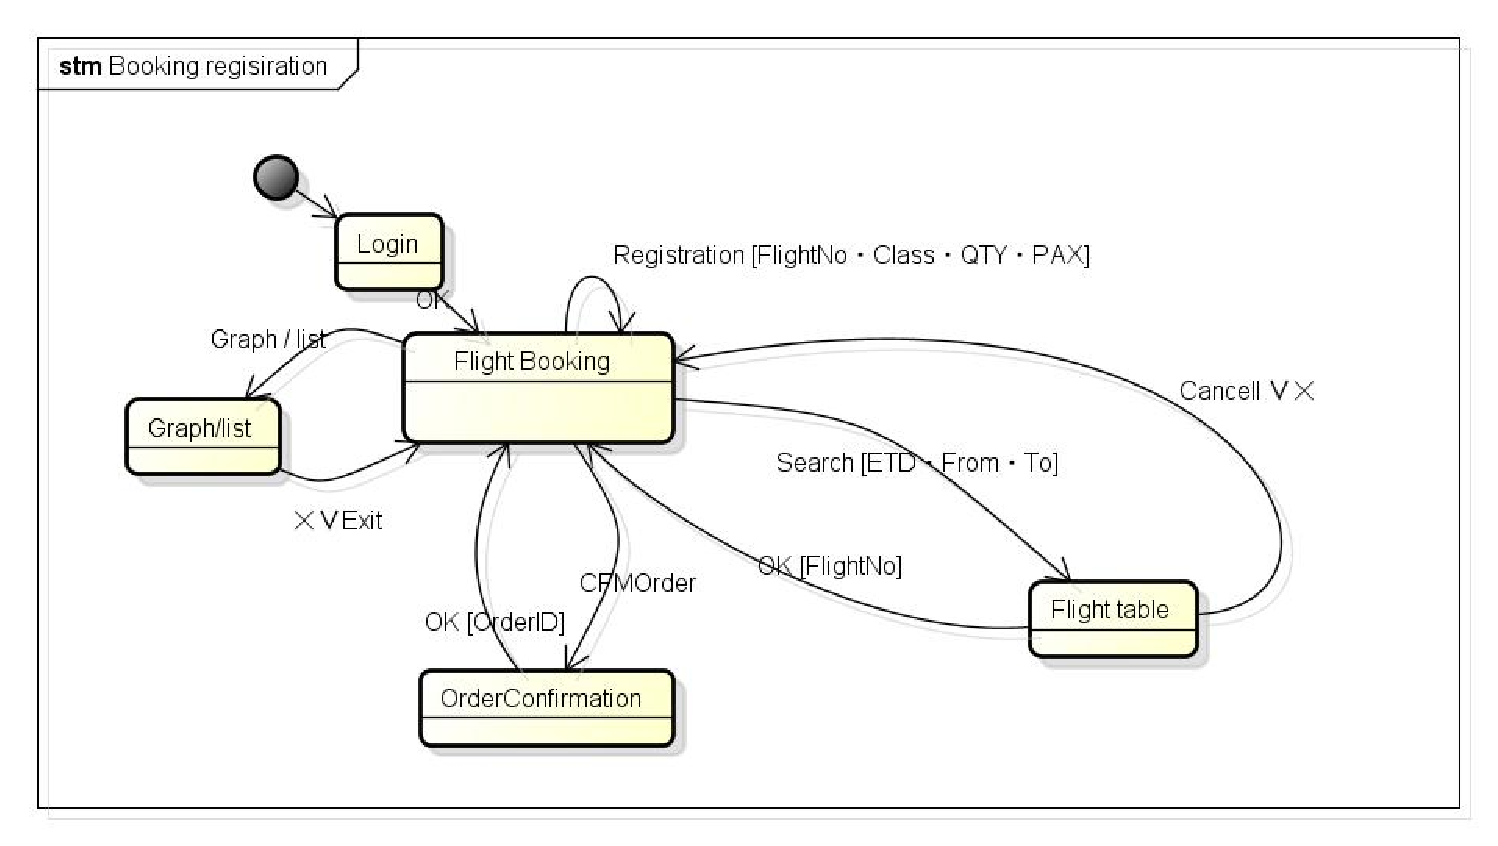
\includegraphics[scale=0.3]{screentransition.eps}
\end{center}
\caption{フライト予約システムの画面遷移図(一部分)}
\label{fig:STD}
\end{figure}

次に提案手法で抽出したタスク間の順序組合せと既出の状態を含む$AP$のテストケースを設計する手法である状態遷移テストで,抽出されるテストケースの比較を行う.状態遷移テストのテストベースとなるフライト予約システムの画面遷移図である図~\ref{fig:STD}を使って,順序組合せが確認できる網羅基準であるS1網羅基準を適用する.
図~\ref{fig:STD}は,適用範囲を合わせるために,4章の適用のためのサブセットである新規フライト予約を行うために必要な画面と隣接する画面遷移に該当する範囲の図となっている.
仕様の詳細度合いは,DFD,ER図,CRUD図と画面遷移図では同等にしている.
それは,画面遷移のイベントでのガード条件に記載したデータがDFDのエッジに記載したデータ,ER図のエンティティの属性と一致していることから確認できる.
S1網羅基準を適用すると28の状態遷移パスとなる.
%この表の提案手法の列には,提案手法で抽出した順序組合せに該当する順序組合せを示した.
%状態遷移パスに対応する提案手法で抽出した順序組合せは28のうち,表~\ref{TCLIST2}テストケースNo.1,2,4,5の4つであった.3-25対応
28の状態遷移パスのうち,対応する提案手法で抽出した順序組合せは,表~\ref{TCLIST2}テストケースNo.1,2,4,5の4つであった.
これらは,本状態遷移図のフライト予約状態での登録イベントを起点にするもののみであった.
順序組合せに該当しない状態遷移パスは,互いのタスクで同一のデータを介して処理をするといったことがない.
例えば,フライト検索をした後にキャンセルをするとフライト予約画面に遷移するパスは,前の処理の結果によって影響を及ぼさない.

S1網羅基準では抽出できないが,本手法によって抽出できたテストケースは,No.3の$Ta_2/Ds_1U  \xrightarrow[Ds_1]{} Ta_6U$である.
このテストケースは,必要なテストケースと考えられる.
%提案手法の適用で利用したテストベースでは,変更が入ったサブセットに該当する範囲で用意している.ここでは,新規フライト予約が変更が入ったサブセットになっているため,新規フライト予約に隣接する画面遷移が,該当するテストベースとなっている.3-26対応
4節の適用評価にて利用したテストベースは,変更が入った機能セットに焦点を絞ったものである.
4節では新規フライト予約が該当する。そのため,図5では,新規フライト予約に隣接する画面遷移が,該当するテストベースとなっている.
表~\ref{TCLIST2}のテストケースNo3における波及タスクである$Ta_6U$は,表~\ref{CRUD}から同期処理のタスクであることがわかるが,新規フライト予約とは別の機能セットに含まれるタスクであり,フライト予約画面と隣接する画面遷移図には現れない.
そのため,S1網羅基準では抽出することができない.
%提案手法で検出できた理由は,テストベースであるDFD,ER図,CRUD図では,新規フライト予約と同期処理の間にはデータを介した順序組合せがあることを示しているためである.

\section{おわりに}

%本論文では,状態遷移を持つソフトウェアにおいて,変更による変更波及がデータベースや外部変数などの保持データを介して生ずる場合のテストに関して,その網羅基準と,テストケースを抽出する手法を提案した.3-6対応によって修正
本論文では,状態遷移を持つソフトウェアにおいて,変更による変更波及がデータベースや外部変数などの保持データを介して生ずる場合のテストに関して,その網羅基準と,順序組合せテストケースを抽出する手法としてIDAU法を提案した.
DFD,ER図、CRUD図をテストベースとして,3つのルールを適用することでテストが必要な順序組合せを抽出できることを説明した.
提案した手法で組合せが抽出できることを確認するため,フライト予約システムの仕様を具体例にして適用を行った.
最後に従来手法である画面遷移図からS1網羅基準にて抽出した状態遷移パスと提案手法を比較して,テストケース数の削減ができる効果と,S1レベルの画面遷移の網羅では抽出できないテストケースが抽出できる効果を示した.

提案手法に対する今後の取り組みは2つある.
1つは,適用範囲の明確化である.変更のパターン(タスク内の制御ロジックの変更,新しい要素の追加など)に対して,どこまで適用でき,どこからは適用できないかを明らかにする.

もう1つは,今回の提案手法のツール化である.
実際の開発プロジェクトで扱う規模の大きいデータ設計文書に対して本手法を適用する際には,本手法のルールをツール化するといった方法での適用が必要になる.
これらの準備を行い,実践の場に本手法を適用していく.

%%%%%%%%%%%%%%%%%%%%%%%
\chapter{結論}

%%%%%%%%%%%%%%%%%%%%%%%

\chapter*{謝辞}
\addcontentsline{toc}{chapter}{\numberline{}謝辞}
入力例


\newpage

\addcontentsline{toc}{chapter}{\numberline{}参考文献}
\renewcommand{\bibname}{参考文献}

%% 参考文献に jbibtex を使う場合
%\bibliographystyle{junsrt}
 \bibliographystyle{sieicej}
\bibliography{mybib1}

% \begin{thebibliography}{1}
% \bibitem{RakRak}
% 野寺隆志.
% \newblock 楽々 \LaTeX.
% \newblock 共立出版, 1990.
% \end{thebibliography}

\end{document}

%%%作業エリア
状態や保持データは,タスク群によって参照,更新されるため,系統的に取り扱う必要がある.
系統的に取り扱う方法としては,状態や保持データのライフサイクルを定義するのが一般的である.
ライフサイクルとは,状態であれば,状態遷移図や状態遷移表によって定義される仕様であり,状態と状態遷移が定められている.
保持データであれば,CRUD図などによりデータの「生成:C」「参照:R」「更新:U」「削除:D」を定義する.
